% !TEX encoding = UTF-8 Unicode
% 부산대학교 pnureport 템플릿 기반, pdfLaTeX 전용
\documentclass[titlepage]{pnureport}

\usepackage[T1]{fontenc}
\usepackage{booktabs}
\usepackage{tabularx}
\usepackage{longtable}
\usepackage{array}
\usepackage{multirow}
\usepackage{graphicx}
\usepackage{float}
\usepackage{subcaption}
\usepackage[table]{xcolor}
\usepackage{enumitem}
\usepackage[hidelinks]{hyperref}
\usepackage{url}

\graphicspath{{figures/}}
\hypersetup{
  pdftitle={3DGS 기반 공간 데이터 시각화 중간보고서},
  pdfauthor={이거왜됨연구회},
  pdfsubject={2026 전기 졸업과제 중간보고서},
  pdfkeywords={3D Gaussian Splatting, PGSR, Sionna RT, ESP32, MQTT, RF Visualization}
}

\definecolor{donegreen}{RGB}{225,242,231}
\definecolor{progressyellow}{RGB}{255,244,204}
\definecolor{pendingred}{RGB}{252,228,228}
\definecolor{headerblue}{RGB}{222,235,247}

\newcommand{\done}{\cellcolor{donegreen}\textbf{완료}}
\newcommand{\statuspartial}{\cellcolor{progressyellow}\textbf{부분 검증}}
\newcommand{\pending}{\cellcolor{pendingred}\textbf{예정}}
\newcommand{\code}[1]{\texttt{#1}}
\newcommand{\source}[1]{\par\smallskip{\footnotesize\color{gray}자료: #1}\par}
\newcolumntype{Y}{>{\raggedright\arraybackslash}X}
\newcolumntype{C}[1]{>{\centering\arraybackslash}p{#1}}
\renewcommand{\arraystretch}{1.25}
\setlength{\headheight}{14pt}
\setlist[itemize]{leftmargin=1.7em,itemsep=0.25em,topsep=0.3em}
\setlist[enumerate]{leftmargin=1.9em,itemsep=0.25em,topsep=0.3em}
\renewcommand{\listfigurename}{그림 목록}
\renewcommand{\listtablename}{표 목록}

\reporttitle{3DGS 기반 공간 데이터 시각화\\2026 전기 졸업과제 중간보고서}
\reportteam{이거왜됨연구회}
\reportauthor{202355708 이승우\\202355701 강주호\\202355707 이나영}
\reportdate{2026년 7월 16일}
\reportadvisor{박영진}

\begin{document}

\hypersetup{pageanchor=false}
\maketitle

\pagenumbering{roman}
\hypersetup{pageanchor=true}
\tableofcontents
\clearpage
\listoffigures
\clearpage
\listoftables
\clearpage

\chapter*{요약}
\addcontentsline{toc}{chapter}{요약}

본 과제는 실제 실내 공간을 3차원으로 재구성하고, 여러 계측 장치가 측정한 와이파이 신호 세기와 전파 시뮬레이션 결과를 공간 구조 위에 겹쳐 보여 주는 통합 시스템을 개발한다. 착수 단계에서는 3차원 가우시안 장면 위에 측정값을 보간한 3차원 신호장을 표현하는 방향을 제안하였다. 중간 단계에서는 구현 위험과 검증 가능성을 고려하여 역할을 더 명확히 분리하였다. 화면용 장면은 3차원 가우시안 표현을 사용하고, 전파 계산은 삼각형 표면 모델을 사용하며, 실시간 실행 중에는 미리 계산한 단일 높이 전파 지도를 읽어 표시하는 구조를 우선한다.

보고 시점까지 그래픽스 파트는 강의실 사진 205장을 이용한 PGSR 장면과 표면 모델을 확보하고, 전파 계산용 닫힌 방 모델과 미터 단위 좌표 변환, Sionna RT 장면 변환을 구현하였다. 2.4 GHz 조건의 저해상도 지도에서 방 내부 151개 셀 모두 유효한 값을 얻었고, 검증용 가상 벽을 추가한 A/B 시험에서는 직접 경로가 제거되며 최대 8.426 dB의 차이가 발생함을 확인하였다. 다만 현재 배율과 재질은 사진 추정 및 기본 재질에 기반하므로 실제 전파 정확도를 입증한 결과는 아니다.

네트워크 파트는 Mosquitto, 백엔드, PostgreSQL, WebSocket으로 이어지는 수집-검증-동기화-저장-전달 경로를 구현하였다. 실물 장치 연동에서 수신된 708건을 백엔드 드롭 없이 저장하고 155개 동기화 프레임을 생성하였다. 모의 부하 시험에서는 노드 12개가 초당 총 120건을 발행하는 조건에서도 백엔드 수신 손실률 0\%와 평균 약 86 ms의 수집 지연을 기록하였다. 임베디드 파트는 ESP32 원격 노드, ESP32 게이트웨이, STM32 수신부, PC 시리얼-MQTT 브리지를 구현하고 빌드 및 호스트 파서 시험을 통과하였다. 그러나 3개 이상 실물 노드의 장시간 시험, 자동 재연결, 핸드헬드 IMU/LCD, 최종 Viewer 합성 및 영상 전송은 남아 있다.

따라서 현재 성과는 ``각 파트의 핵심 기술 검증과 계측 데이터의 서버 종단 연결''까지로 평가한다. 최종 목표인 ``실제 측정값과 전파 지도를 3DGS Viewer에 합성하여 핸드헬드 장치로 실시간 표시''는 아직 달성하지 않았다. 이후에는 현장 실측을 통한 좌표/재질 보정, 다중 실물 노드 안정성 시험, SIBR Viewer 합성, JPEG 스트리밍과 핸드헬드 표시를 순서대로 통합한다.

\clearpage
\pagenumbering{arabic}

\chapter{프로젝트 개요}

\section{개발 배경과 문제 정의}

실내 와이파이 품질은 송신기와 수신기 사이 거리뿐 아니라 벽, 문, 가구, 재질, 높이와 같은 공간 요소의 영향을 받는다. 그러나 일반적인 수치 목록이나 평면 히트맵은 어느 위치의 신호가 약한지는 보여 주어도, 실제 공간의 어떤 구조가 감쇠와 차폐를 만들었는지는 직관적으로 설명하기 어렵다. 본 과제는 이 문제를 해결하기 위해 실제 공간의 시각적 모습, 전파 계산 결과, 실측 RSSI(Received Signal Strength Indicator)를 하나의 좌표계에서 연결한다.

화면 표현에는 사진으로부터 실제 장면을 빠르게 재구성하고 새로운 시점에서 실시간에 가깝게 렌더링할 수 있는 3D Gaussian Splatting(3DGS)을 사용한다\cite{kerbl2023}. 다만 일반 3DGS는 시각적 렌더링에 최적화된 가우시안 집합이므로 전파 경로가 부딪히는 명시적 표면으로 바로 사용하기 어렵다. 이에 평면 기반 제약과 편향 없는 깊이를 이용해 표면 복원을 강화한 PGSR을 우선 재구성 경로로 선택하였다\cite{chen2024pgsr}.

\section{개발 목표}

최종 시스템의 목표는 다음 세 가지다.

\begin{enumerate}
  \item 실제 강의실을 3DGS 장면으로 재구성하고, 전파 계산에 사용할 표면 모델과 동일 좌표계로 관리한다.
  \item 여러 임베디드 노드의 RSSI를 안정적으로 수집, 검증, 시간 동기화하여 그래픽스 파트가 즉시 사용할 수 있는 프레임으로 제공한다.
  \item 미리 계산한 전파 지도와 실측값을 3DGS 장면에 합성하고, 사용자의 시점에 맞춰 렌더링한 화면을 핸드헬드 장치에 전달한다.
\end{enumerate}

\section{전체 시스템 구조}

전체 시스템은 오프라인 구축과 실시간 실행으로 구분한다. 오프라인에서는 사진 촬영, 카메라 자세 추정, PGSR 학습, 표면 모델 보정, Sionna RT 전파 지도 계산을 수행한다. 실시간에서는 임베디드 노드가 RSSI와 상태를 보내고, 백엔드가 이를 동기화하며, Viewer가 저장된 전파 지도와 최신 측정값을 장면에 합성한다. 장면과 송신기, 주파수, 재질이 고정되어 있는 동안 Sionna RT를 매 화면마다 다시 실행하지 않는다. Sionna RT의 Radio Map은 한 평면의 위치별 path gain, RSS 또는 SINR을 계산할 수 있으므로\cite{aitaoudia2025sionna}, 본 과제의 최소 구현에서는 사람이 장치를 드는 높이의 단일 2차원 지도를 3차원 공간에 배치한다.

\begin{table}[H]
\centering
\caption{시스템 계층별 입력, 처리, 출력}
\label{tab:system-layers}
\begin{tabularx}{\textwidth}{C{2.4cm}YYY}
\toprule
계층 & 주요 입력 & 핵심 처리 & 주요 출력 \\
\midrule
임베디드 & AP 신호, 노드 상태 & 측정, 이동평균, 오류 검출, 패킷화 & RSSI 패킷, 상태 정보 \\
네트워크/백엔드 & MQTT 메시지 & 검증, 200 ms 동기화, 저장, 모니터링 & WebSocket 프레임, REST 지표 \\
그래픽스/전파 & 사진, PGSR Mesh, 위치, RSSI & 장면 재구성, 좌표 보정, 전파 계산, 합성 & 3DGS 장면과 전파 히트맵 \\
핸드헬드 & IMU, 버튼, JPEG 스트림 & 방향 입력, 위치 갱신 요청, 영상 복호화 & 800$\times$480 LCD 화면 \\
\bottomrule
\end{tabularx}
\end{table}

\section{중간보고 범위와 판단 기준}

본 보고서는 2026년 7월 15일 회의 자료와 7월 14일 기준 세 저장소의 구현 상태를 중심으로 작성하였다\cite{rfvisualizerRepo,networkRepo,embeddedRepo}. 파일이나 코드가 존재하는 것만으로 완료 처리하지 않고, 다음 기준을 구분한다.

\begin{itemize}
  \item \textbf{완료}: 실제 입력이나 재현 가능한 시험으로 출력까지 확인한 기능
  \item \textbf{부분 검증}: 단위 기능, 빌드, 모의 입력 또는 제한된 장치에서 확인했으나 최종 환경 검증이 남은 기능
  \item \textbf{예정}: 설계만 확정되었거나 구현을 시작하지 않은 기능
\end{itemize}

\chapter{요구조건 및 제약 사항의 수정}

\section{착수 계획 대비 핵심 변경}

착수보고서는 다중 ESP32의 RSSI를 MQTT로 수집하고 3DGS 장면에서 3차원 신호장으로 표현하는 큰 방향을 제시하였다. 중간 구현에서는 파트 간 연결을 실제로 시험하면서 표 \ref{tab:requirement-changes}와 같이 범위를 수정하였다. 변경의 원칙은 핵심 기능을 삭제하는 것이 아니라, 실패 가능성이 큰 연결부를 작은 검증 단위로 나누는 것이다.

\begin{longtable}{C{2.5cm}p{4.2cm}p{5.7cm}}
\caption{착수 계획 대비 요구조건과 설계 변경}\label{tab:requirement-changes}\\
\toprule
항목 & 착수 단계 & 중간 단계의 수정 및 이유 \\
\midrule
\endfirsthead
\toprule
항목 & 착수 단계 & 중간 단계의 수정 및 이유 \\
\midrule
\endhead
신호장 표현 & 여러 지점의 RSSI를 보간한 3차원 히트맵과 볼륨 렌더링 & 먼저 단일 높이의 2차원 Radio Map을 3차원 공간에 배치한다. 계산량과 가림 처리 위험을 줄이고 파트 연결을 먼저 검증하기 위함이다. \\
전파 계산 & 측정값과 공간 구조를 결합한 RF Field & PGSR Mesh에서 닫힌 Proxy Mesh를 만들고 Sionna RT로 경로와 지도를 미리 계산한다. 실제 측정값은 이후 검증 및 보정 입력으로 사용한다. \\
장면 표현 & 3DGS 장면을 재구성해 시각화 & 화면은 3DGS, 전파 계산은 Triangle Mesh로 역할을 분리한다. 가우시안의 시각 품질과 메시의 명시적 교차 계산을 각각 활용한다. \\
고정 노드 전송 & 각 ESP32가 Wi-Fi/MQTT로 직접 발행 & ESP32 원격 노드가 ESP-NOW로 게이트웨이에 전송하고, STM32 전처리와 PC 브리지를 거쳐 MQTT로 발행한다. 다중 노드 무선 처리와 MCU 전처리를 분리해 시험하기 위함이다. \\
MQTT 브로커 & Python 기반 개발용 브로커 사용 가능 & 원격 발행 전달 문제를 확인한 뒤 Mosquitto로 교체했다. 다중 장치 LAN 연결과 운영 표준에 맞추기 위함이다. \\
위치/방향 & 고정 위치 메타데이터 중심 & 메시지에 선택적 위치와 쿼터니언 회전 필드를 추가했다. 핸드헬드 위치는 연속 추적보다 버튼을 눌렀을 때 갱신하는 방식을 우선 검토한다. \\
핸드헬드 & 현장에서 상태와 최종 결과를 표시 & IMU, 버튼, LCD, JPEG 스트리밍을 고위험 후속 단계로 분리한다. LCD가 목표 성능에 미달하면 PC Viewer를 시연 대안으로 사용한다. \\
실시간 Viewer & 일반 3차원 Viewer에서 결과 표시 & 공식 3DGS SIBR 실시간 Viewer를 먼저 확장한다. 기존 카메라와 가우시안 렌더러를 유지하고 전파 지도, 깊이, 통신을 별도 모듈로 추가한다. \\
\bottomrule
\end{longtable}

\section{그래픽스 및 전파 계산의 제약}

PGSR은 시각적으로 자연스러운 메시를 제공하지만, 천장과 벽에 구멍이나 노이즈가 남아 전파 계산의 닫힌 경계로 바로 사용하기 어렵다. 따라서 바닥, 천장, 벽의 큰 평면을 검출하고 사람이 후보를 선택해 닫힌 방 껍질을 만드는 Proxy Mesh 경로를 추가하였다. 이 과정은 계산 가능성을 높이지만 원본 공간의 세부 구조를 단순화한다.

현재 미터 배율은 사진 속 문의 크기로 추정한 임시값이다. 추정 기준 두 개의 배율 차이가 약 8.15\%이므로 실제 줄자 또는 레이저 거리계 측정 전에는 물리적으로 검증된 크기로 간주할 수 없다. 또한 Sionna RT 장면은 2.4 GHz에서 기본 콘크리트/목재 재질을 사용하며, 실제 벽체의 유전율과 전도도를 측정한 값이 아니다. 따라서 현재의 dB 값은 파이프라인과 상대 변화 검증용이며, 실제 RSSI 예측 정확도를 주장하지 않는다.

\section{임베디드 및 네트워크의 제약}

ESP-NOW와 와이파이 스캔은 동일 채널 운영이 필요하므로 목표 AP와 노드 설정을 함께 관리해야 한다. 현재 초기 설정은 SSID와 채널 6을 기준으로 하며, 같은 SSID를 가진 AP가 여러 개이면 다른 AP를 측정할 수 있다. 최종 실험에서는 BSSID와 실제 게이트웨이 MAC 주소를 고정하고, broadcast와 unicast의 성공률을 비교해야 한다. ESP-NOW는 ESP32 장치 간 직접 통신을 위한 API를 제공하지만\cite{espressifEspnow}, 현장 품질은 채널 혼잡과 노드 배치에 따라 달라지므로 실물 시험이 필수다.

MQTT는 제한된 장치와 불안정한 네트워크에 적합한 경량 발행/구독 방식이다\cite{mqttStandard}. 현재 개발 구성은 익명 접속을 허용하므로 시연 전 계정 인증과 방화벽 정책이 필요하다. 학교 공용 와이파이는 장치 간 직접 통신을 막는 AP isolation이 있어 개인 공유기 기반 동일 LAN을 사용하였다. 이는 기능 검증에는 적합하지만 최종 시연 네트워크의 주소, DHCP 예약, 포트 정책을 사전에 고정해야 한다.

\chapter{시스템 설계 상세화}

\section{그래픽스 오프라인 구축 파이프라인}

그래픽스 파트는 시각화용 장면과 전파 계산용 표면을 함께 얻기 위해 PGSR을 사용한다. PGSR은 가우시안을 표면에 가까운 평면 형태로 정렬하고, 거리와 법선 지도를 이용한 편향 없는 깊이와 다중 시점 일관성 제약을 제공한다\cite{chen2024pgsr}. 본 프로젝트의 오프라인 흐름은 다음과 같다.

\begin{enumerate}
  \item 강의실을 여러 방향에서 촬영하고 COLMAP으로 카메라 자세와 희소 점군을 계산한다.
  \item PGSR을 학습해 3DGS 장면, 깊이, 표면 Mesh를 생성한다.
  \item 표면 Mesh에서 큰 평면 후보를 검출하고 바닥, 천장, 벽을 선택한다.
  \item 선택한 평면의 교차점으로 경계 모서리를 계산해 구멍 없는 Room Envelope를 만든다.
  \item 장면 좌표를 미터 단위 좌표로 변환하고, 전파 재질을 연결한 Mitsuba/Sionna 장면을 생성한다.
  \item 송신기 위치와 수신 높이를 정한 뒤 경로와 단일 높이 Radio Map을 계산해 파일로 저장한다.
\end{enumerate}

\begin{figure}[H]
\centering
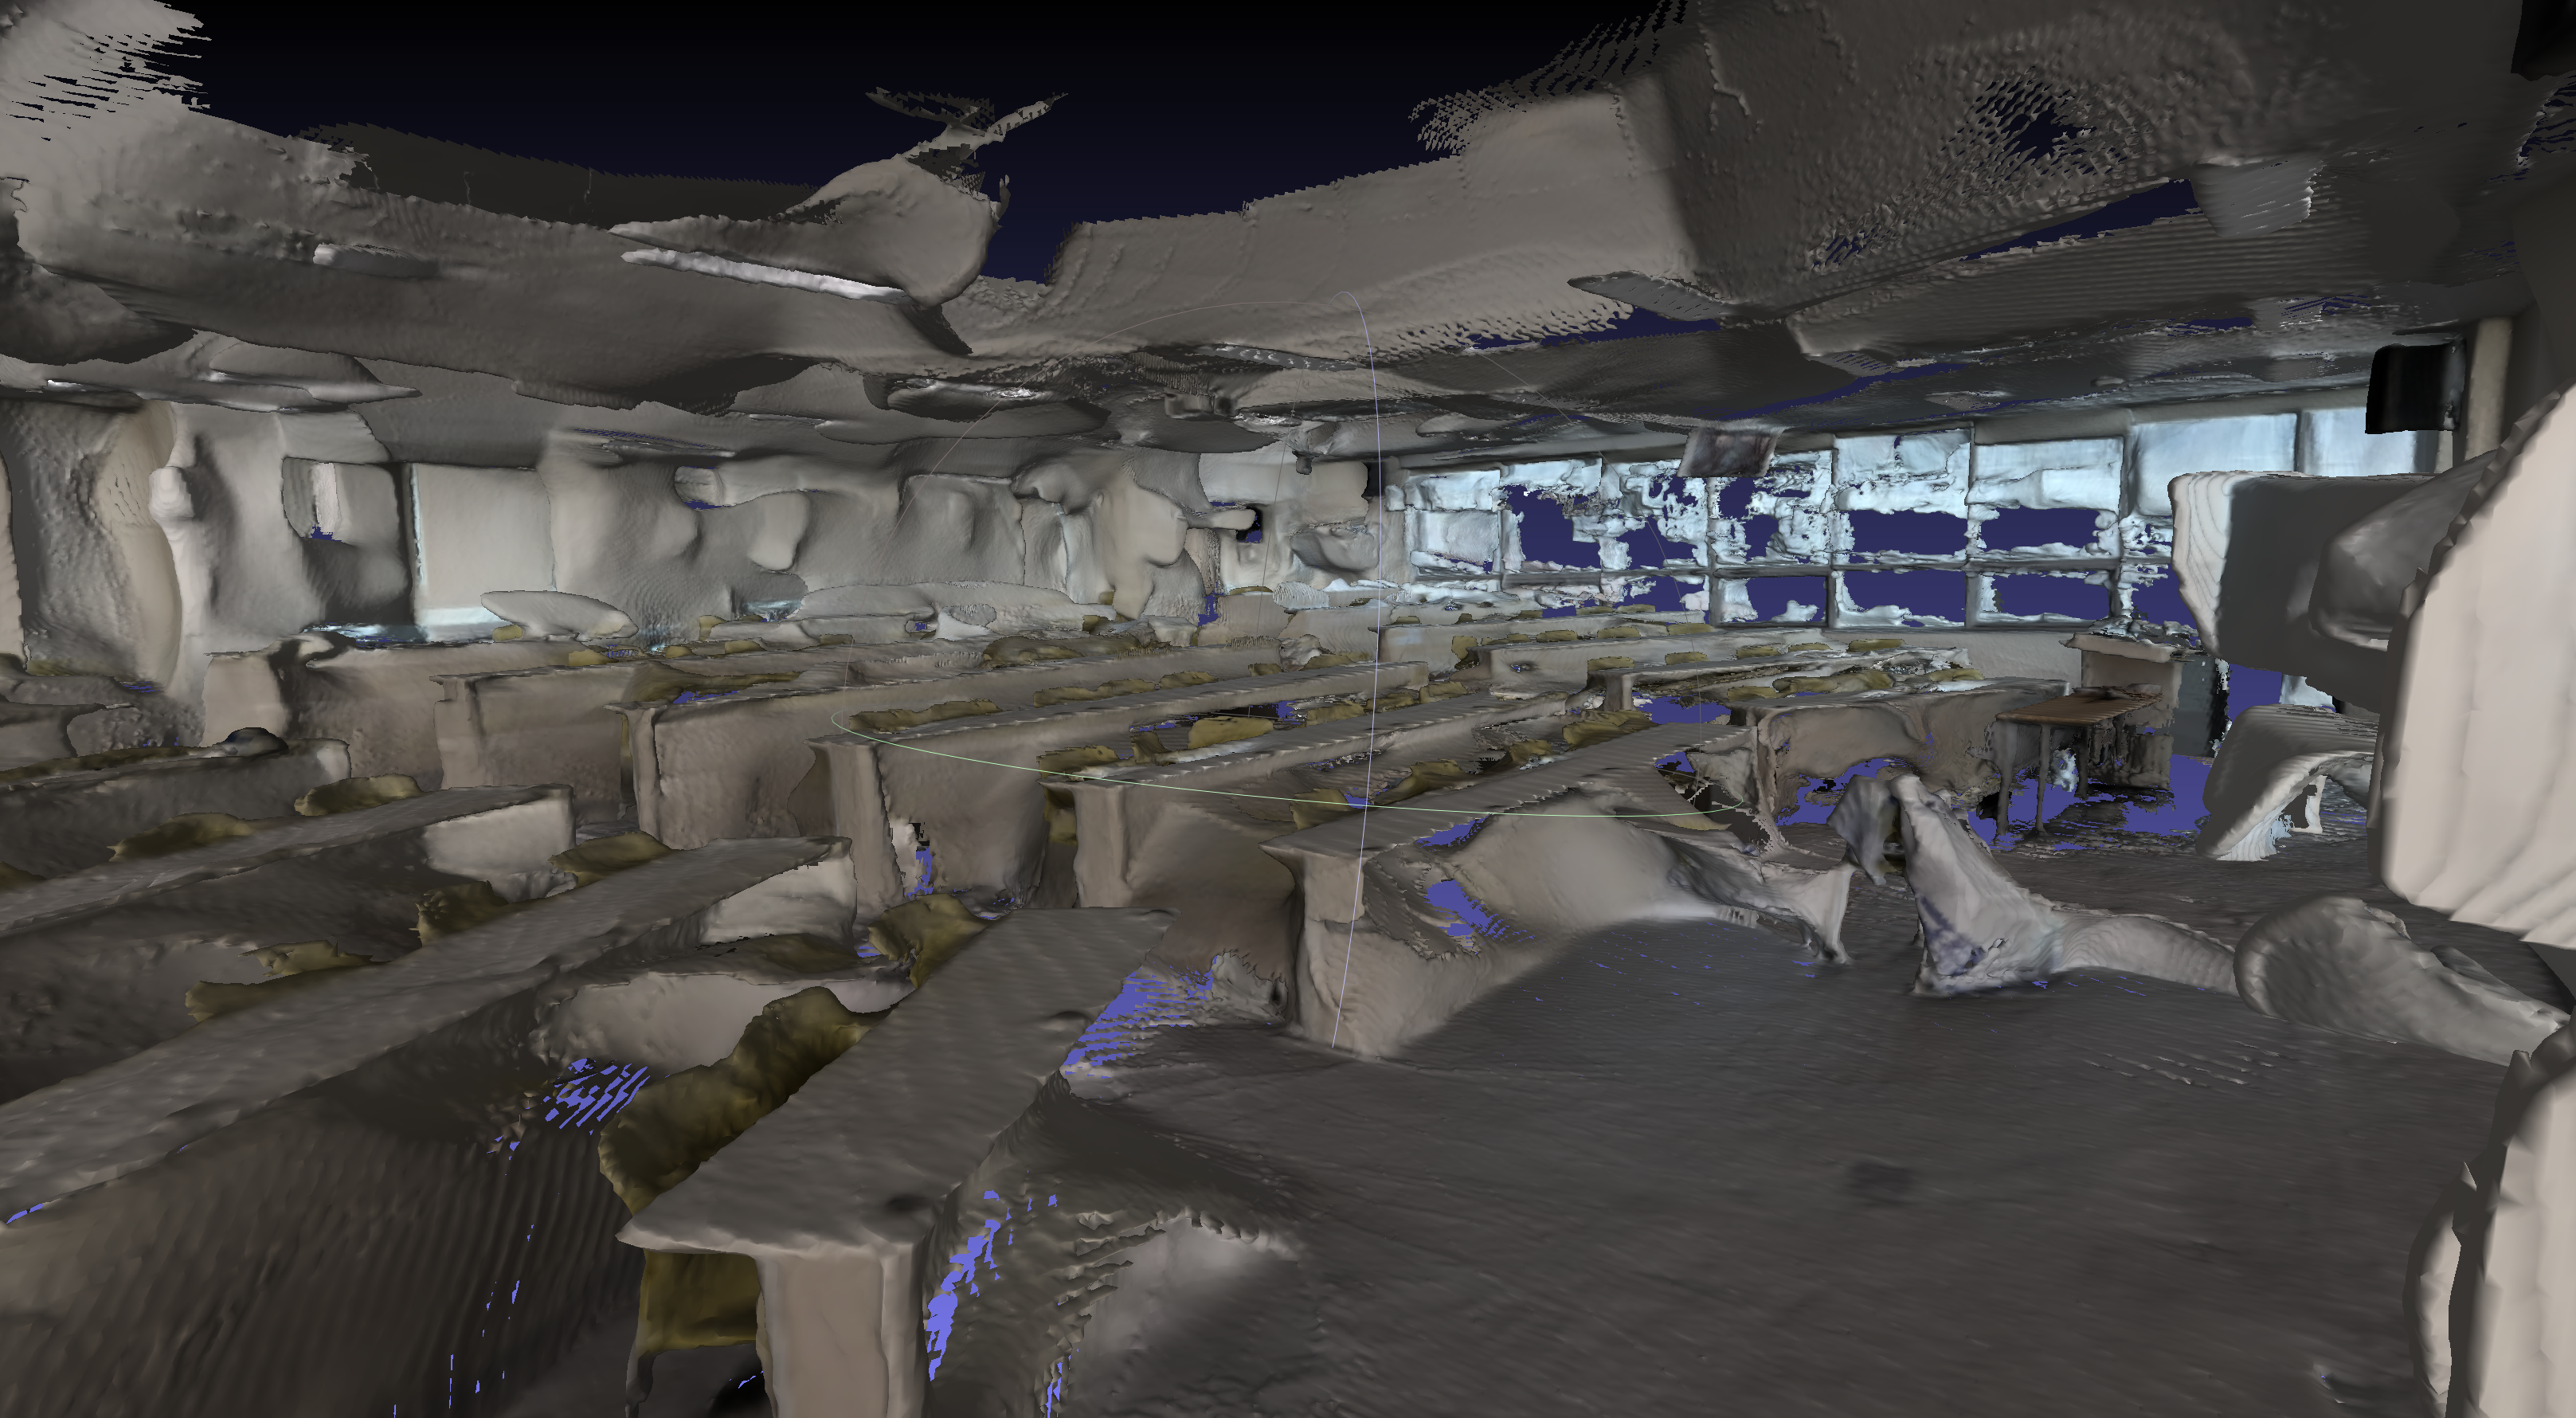
\includegraphics[width=0.96\textwidth]{pgsr_mesh.png}
\caption{PGSR에서 추출한 강의실 표면 Mesh. 책상과 벽의 형태는 보이지만 천장과 창 주변의 구멍 및 노이즈가 남아 있어 전파 계산용 단순화가 필요하다.}
\label{fig:pgsr-mesh}
\end{figure}

\begin{figure}[H]
\centering
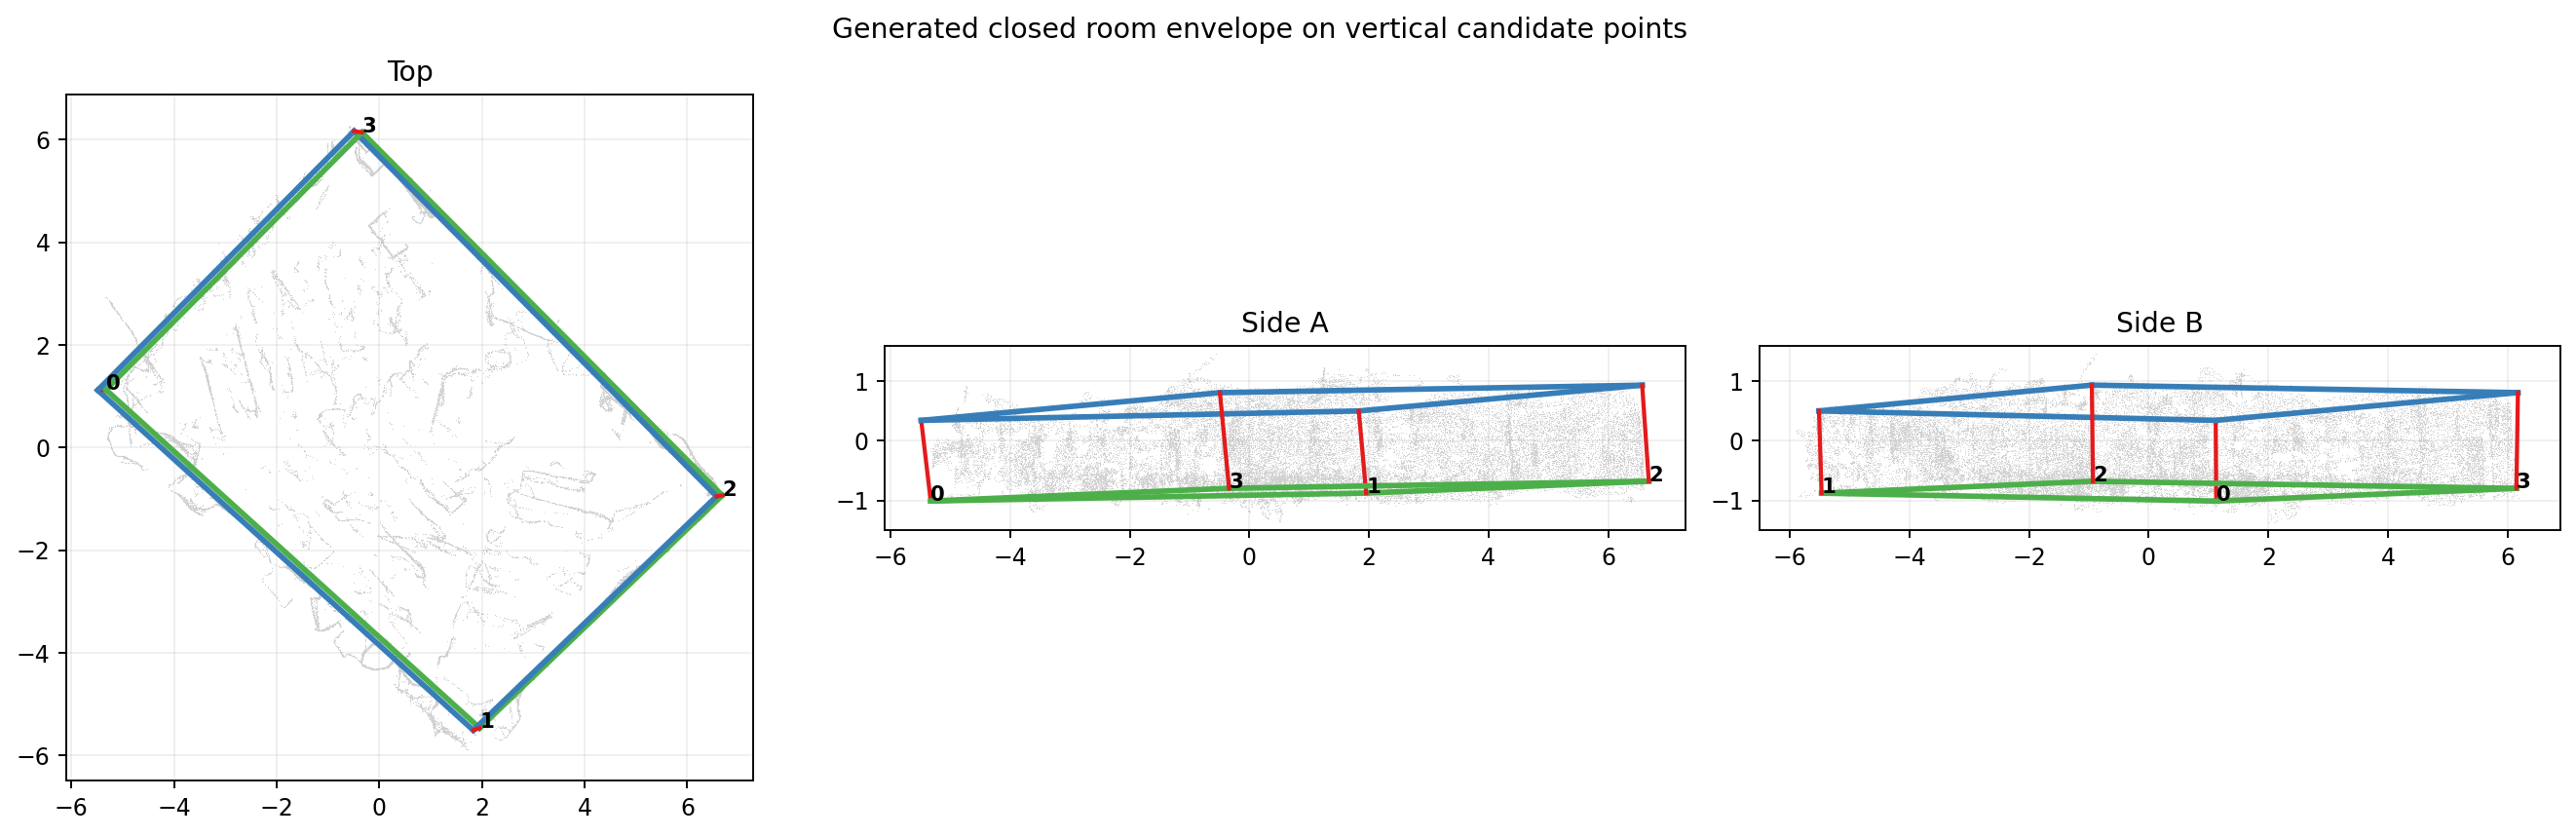
\includegraphics[width=0.98\textwidth]{room_envelope.png}
\caption{검출한 평면 후보를 이용해 생성한 닫힌 Room Envelope의 위/옆 투영}
\label{fig:room-envelope}
\end{figure}

\section{임베디드 계측 파이프라인}

원격 ESP32 노드 1--4는 목표 AP의 RSSI를 200 ms마다 측정하고 최근 5개 유효값의 이동평균을 만든다. 1초마다 노드 ID, 순번, 원시/필터 RSSI, 오류 상태와 CRC32를 포함한 ESP-NOW 패킷을 게이트웨이에 전송한다. 게이트웨이는 원격 노드의 CRC, 중복, 누락을 검사하며 자체 RSSI를 로컬 노드 5로 추가한다.

게이트웨이는 측정값을 115200 bps UART Line으로 STM32 보드에 전달한다. STM32는 인터럽트 기반으로 바이트를 수신하고 체크섬과 형식을 검사한다. 또한 노드별 최신값과 타임아웃 상태를 관리해 MQTT 발행용 JSON을 생성한다. 현재 최종 네트워크 인터페이스가 확정되지 않아 PC의 시리얼-MQTT 브리지가 JSON을 정규화하고 설치 좌표를 결합한 뒤 MQTT로 발행한다.

\begin{figure}[H]
\centering
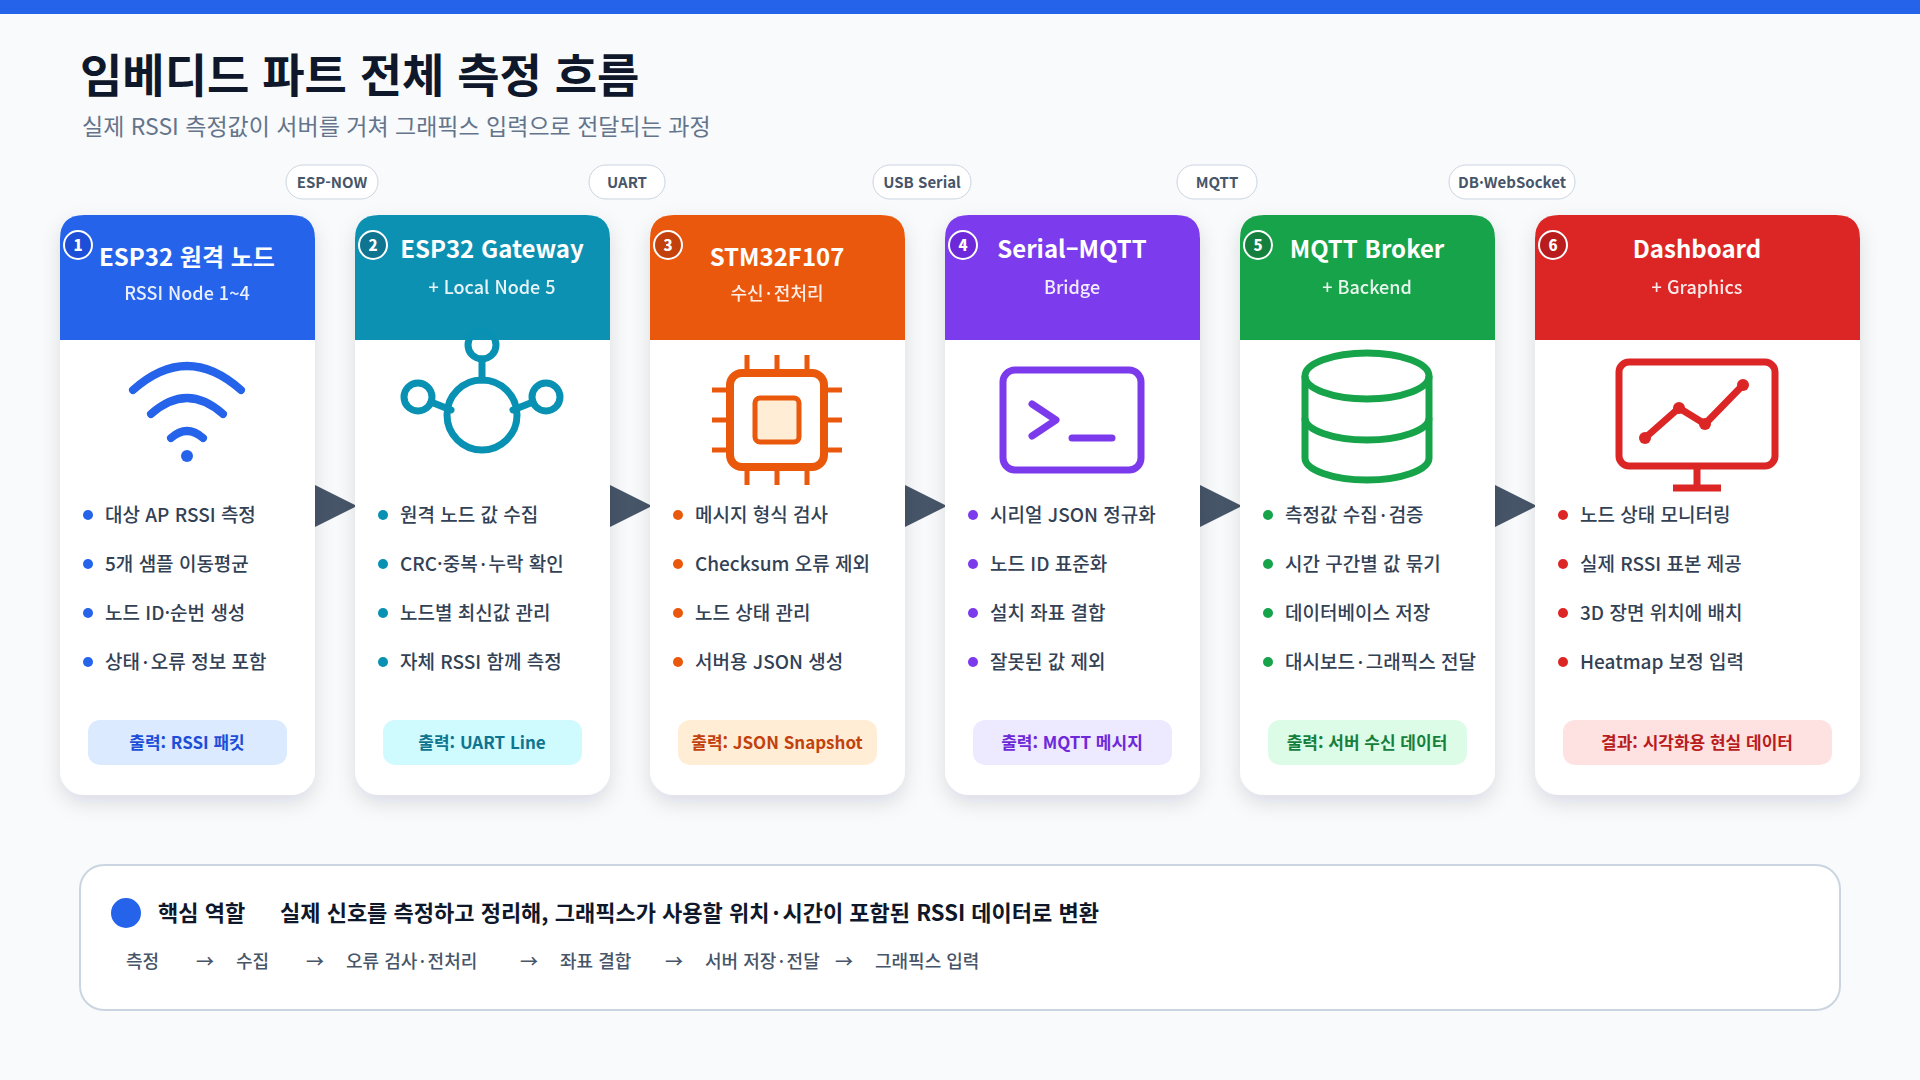
\includegraphics[width=\textwidth]{embedded_flow.png}
\caption{임베디드 측정값이 그래픽스 입력으로 전달되는 전체 경로}
\label{fig:embedded-flow}
\end{figure}

\section{네트워크 및 백엔드 파이프라인}

백엔드는 Mosquitto 브로커에서 개별 노드 토픽과 게이트웨이 묶음 토픽을 구독한다. 수신 데이터는 JSON 형식, 필수 필드, RSSI 범위($-100$--$-10$ dBm), 타임스탬프를 검사한다. 노드별 순번으로 송신 구간의 누락을 집계하고, 근접 시각의 값을 200 ms Time Window로 묶어 하나의 프레임으로 만든다.

원시 측정값은 PostgreSQL의 \code{rssi\_raw}에 배치 삽입하고, 동기화 프레임과 노드 상태는 별도 테이블에 저장한다. 최신 프레임은 WebSocket \code{/frames}로 그래픽스에 push하며, \code{/metrics}, \code{/nodes/status}, \code{/health} 등의 REST API로 지표와 상태를 제공한다. 위치와 회전은 임베디드의 평면 필드를 그래픽스가 바로 사용할 수 있는 중첩 객체로 변환한다.

\begin{table}[H]
\centering
\caption{파트 간 핵심 데이터 계약}
\label{tab:data-contract}
\begin{tabularx}{\textwidth}{C{2.4cm}Y Y}
\toprule
구간 & 필수 항목 & 선택/추가 항목 \\
\midrule
임베디드 $\rightarrow$ MQTT & node\_id, timestamp, rssi, seq, status & rssi\_raw, pos\_x/y/z, rot\_w/x/y/z \\
백엔드 내부 & server\_receive\_ms, 유효성, 노드 상태 & 누락 노드, 지연, 드롭/손실 집계 \\
WebSocket $\rightarrow$ 그래픽스 & 노드별 rssi, seq, pos, rot & frame\_timestamp, missing, 서버 지표 \\
\bottomrule
\end{tabularx}
\end{table}

\section{실시간 Viewer와 핸드헬드 설계}

실시간 화면은 공식 SIBR Viewer의 가우시안 렌더링과 카메라 구조를 유지한 채 프로젝트 기능을 별도 모듈로 추가한다. 3DGS 장면은 기존 렌더러가 그리며, PGSR Mesh는 깊이만 기록하는 pass에 사용한다. Radio Map은 반투명 평면 텍스처로 그린 뒤 장면 깊이와 비교해 벽 뒤의 히트맵이 보이지 않도록 합성한다.

렌더링, JPEG 인코딩, TCP 전송, 자세 수신은 독립된 Thread로 분리한다. Frame Queue는 1--2개로 제한하고 오래된 화면을 버려 지연 누적을 막는다. 핸드헬드 ESP32-S3는 3차원 장면을 직접 렌더링하지 않고 IMU 방향과 버튼 입력을 PC에 전송하며, PC가 렌더링한 JPEG를 받아 800$\times$480 LCD에 표시한다. 이 구조는 설계가 확정되었으나 구현 및 성능 검증은 남아 있다.

\chapter{보고 시점까지의 수행 내용과 중간 결과}

\section{그래픽스 파트}

\subsection{장면 재구성과 전파 계산용 기하 생성}

강의실 사진 205장을 사용해 PGSR 장면과 TSDF 후처리 Mesh를 만들었다. 입력 Mesh는 꼭짓점 3,666,424개와 삼각형 6,933,784개로 구성되며, 평면 검출용 전처리 후 194,388점으로 정리하였다. 초기 일반 평면 검출은 수직 후보가 2개에 불과하여, 법선 방향으로 수직 가능점을 먼저 고르는 벽 전용 추출 경로를 추가했고 벽 후보 12개를 얻었다.

사람이 선택한 바닥, 천장, 벽 4개의 무한 평면을 교차해 꼭짓점 8개와 삼각형 12개로 이루어진 닫힌 Room Envelope를 생성하였다. 경계 모서리, 비다양체 모서리, 퇴화 삼각형이 모두 0이며 연결 요소 1개와 Euler characteristic 2를 확인하였다. 이후 사진 속 문 크기로 추정한 단일 배율을 적용해 약 $15.6\times11.1\times3.0$ m 경계의 임시 미터 좌표 장면을 만들었다. 이 크기는 현장 실측 전까지 provisional 상태다.

\subsection{Sionna RT 연결 시험}

Sionna RT는 삼각형 장면과 전파 재질을 이용해 송신기/수신기 사이 경로와 Radio Map을 계산한다\cite{aitaoudia2025sionna}. 본 과제는 Room Envelope를 바닥, 천장, 벽 4개의 총 6개 객체로 변환해 로드하였다. 2.4 GHz, 최대 상호작용 2회 조건에서 4.0 m 직접 경로의 계산 오차는 약 $9.3\times10^{-8}$ m였고, 반사 시험에서는 직접 경로를 포함해 총 26개 경로를 얻었다.

\begin{figure}[H]
\centering
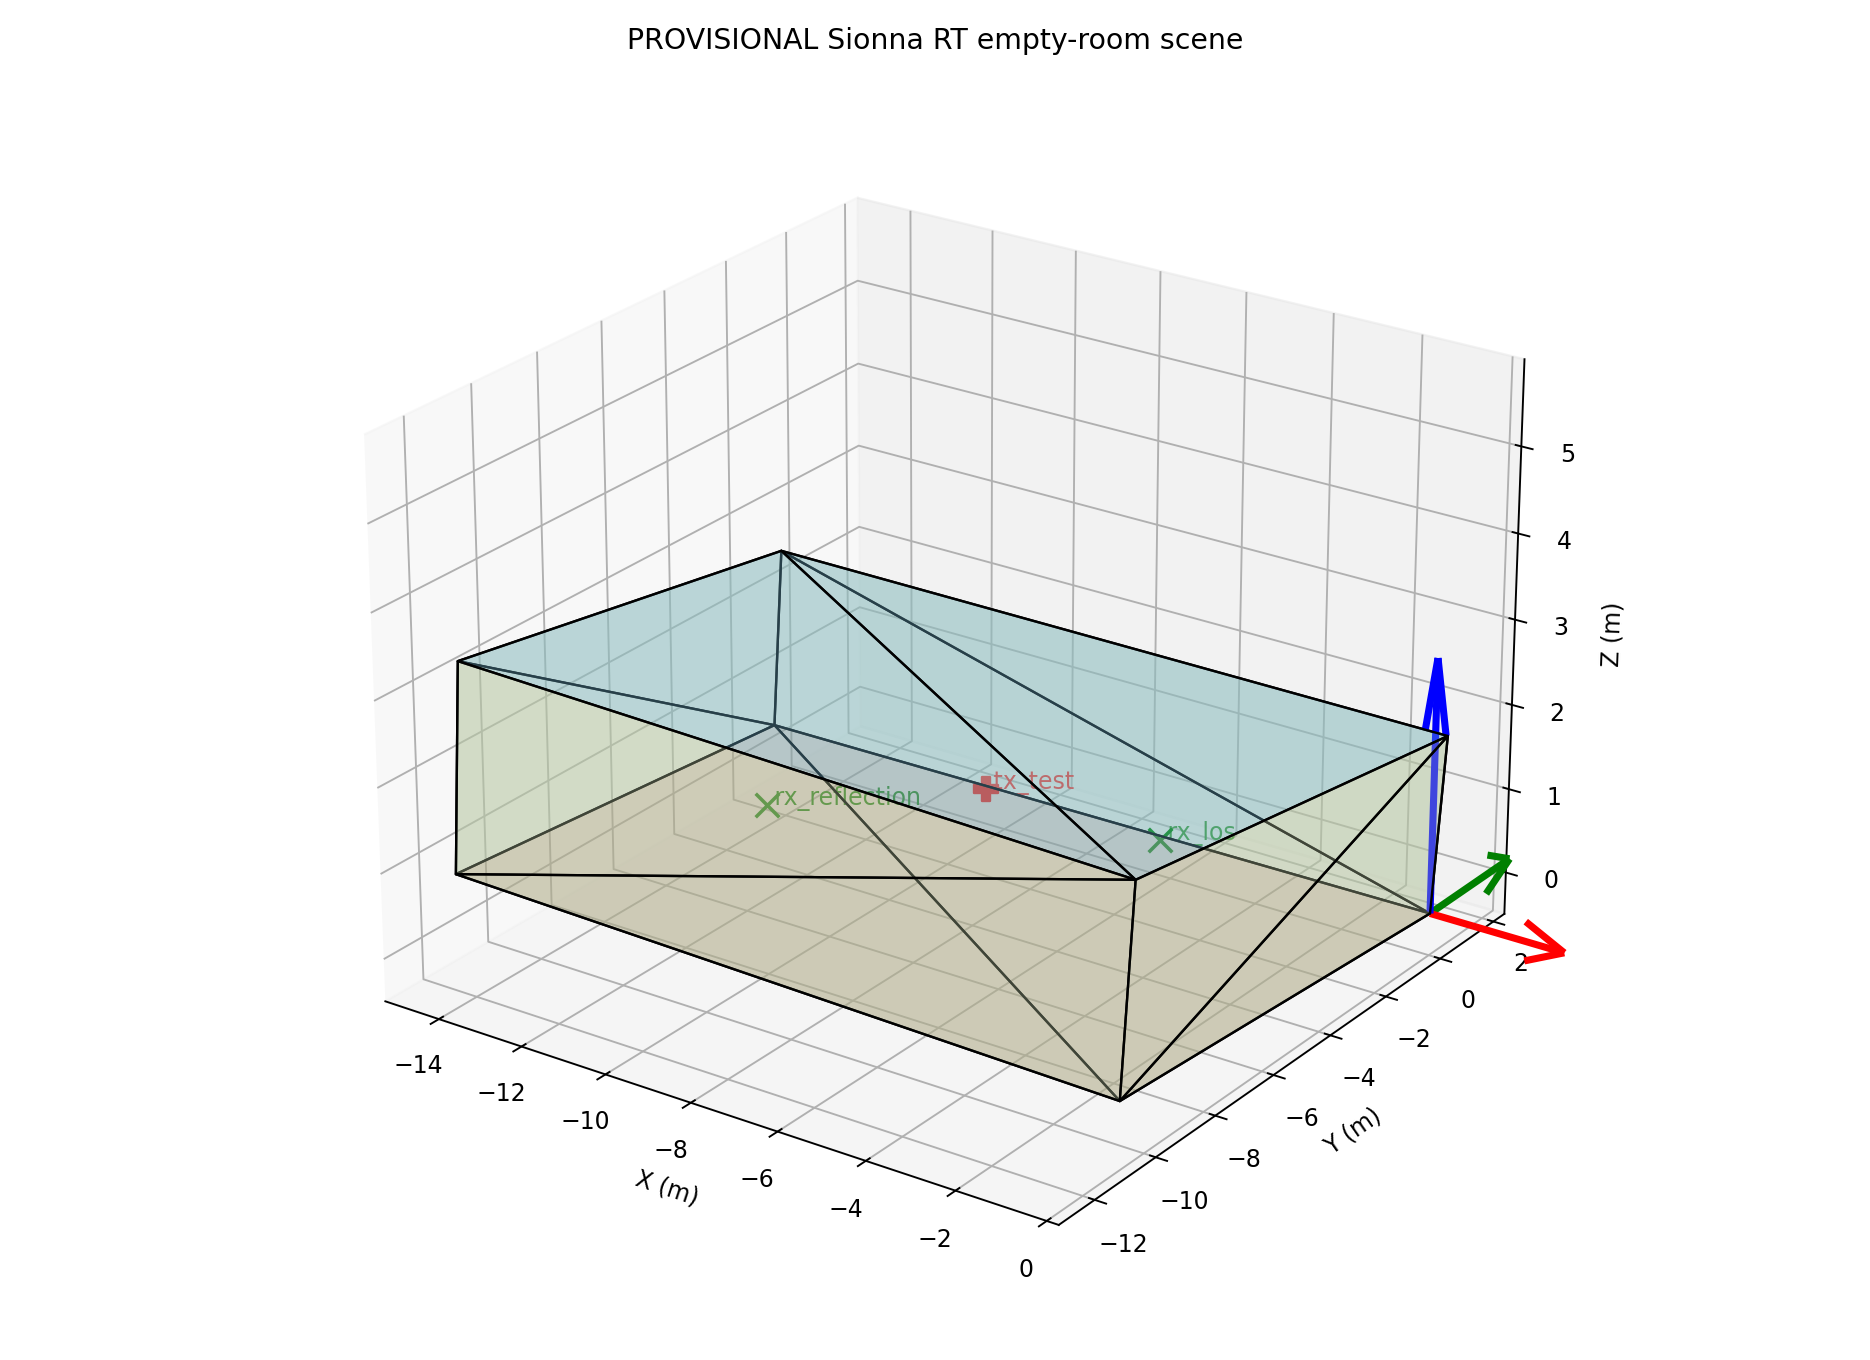
\includegraphics[width=0.83\textwidth]{sionna_scene.png}
\caption{미터 단위 Room Envelope와 송신기/수신기를 배치한 임시 Sionna RT 장면}
\label{fig:sionna-scene}
\end{figure}

높이 1.5 m, 셀 크기 $1\times1$ m의 $11\times15$ 격자에서 전체 165셀 중 방 내부 151셀 모두 유효한 path gain을 얻었다. 최솟값/평균/최댓값은 각각 $-61.064/-58.664/-20.772$ dB였다. 계산 시간은 장면 로드 0.1650초, 직접 경로 0.0718초, 반사 경로 0.0934초, 저해상도 Coverage 0.0044초였다. 이 수치는 RTX 4090과 Sionna RT 1.2.2의 전용 환경에서 측정한 연결 시험 결과다.

\subsection{가상 벽 A/B 시험}

공간 구조가 solver 결과에 실제 영향을 주는지 확인하기 위해 실제 물체가 아닌 검증용 목재 가상 벽을 송신기와 수신기 사이에 추가하였다. 같은 송신기/수신기, seed, solver, 격자를 사용해 empty baseline을 2회 반복하고 variant를 1회 실행하였다. 그 결과 대상 수신기의 직접 경로가 1개에서 0개로 사라졌고, 두 수신기를 합친 전체 경로는 53개에서 35개로 감소하였다.

151개 공통 유효 셀의 평균 변화는 $-1.012$ dB, 최대 절대 변화는 8.426 dB였다. $|\Delta|>1$ dB인 셀은 48개, $|\Delta|>3$ dB인 셀은 6개였다. baseline 반복 차이의 최대값은 $5.20\times10^{-6}$ dB이므로 구조물 추가에 따른 변화가 수치 잡음보다 충분히 큼을 확인하였다.

\begin{figure}[H]
\centering
\begin{subfigure}[b]{0.32\textwidth}
  \centering
  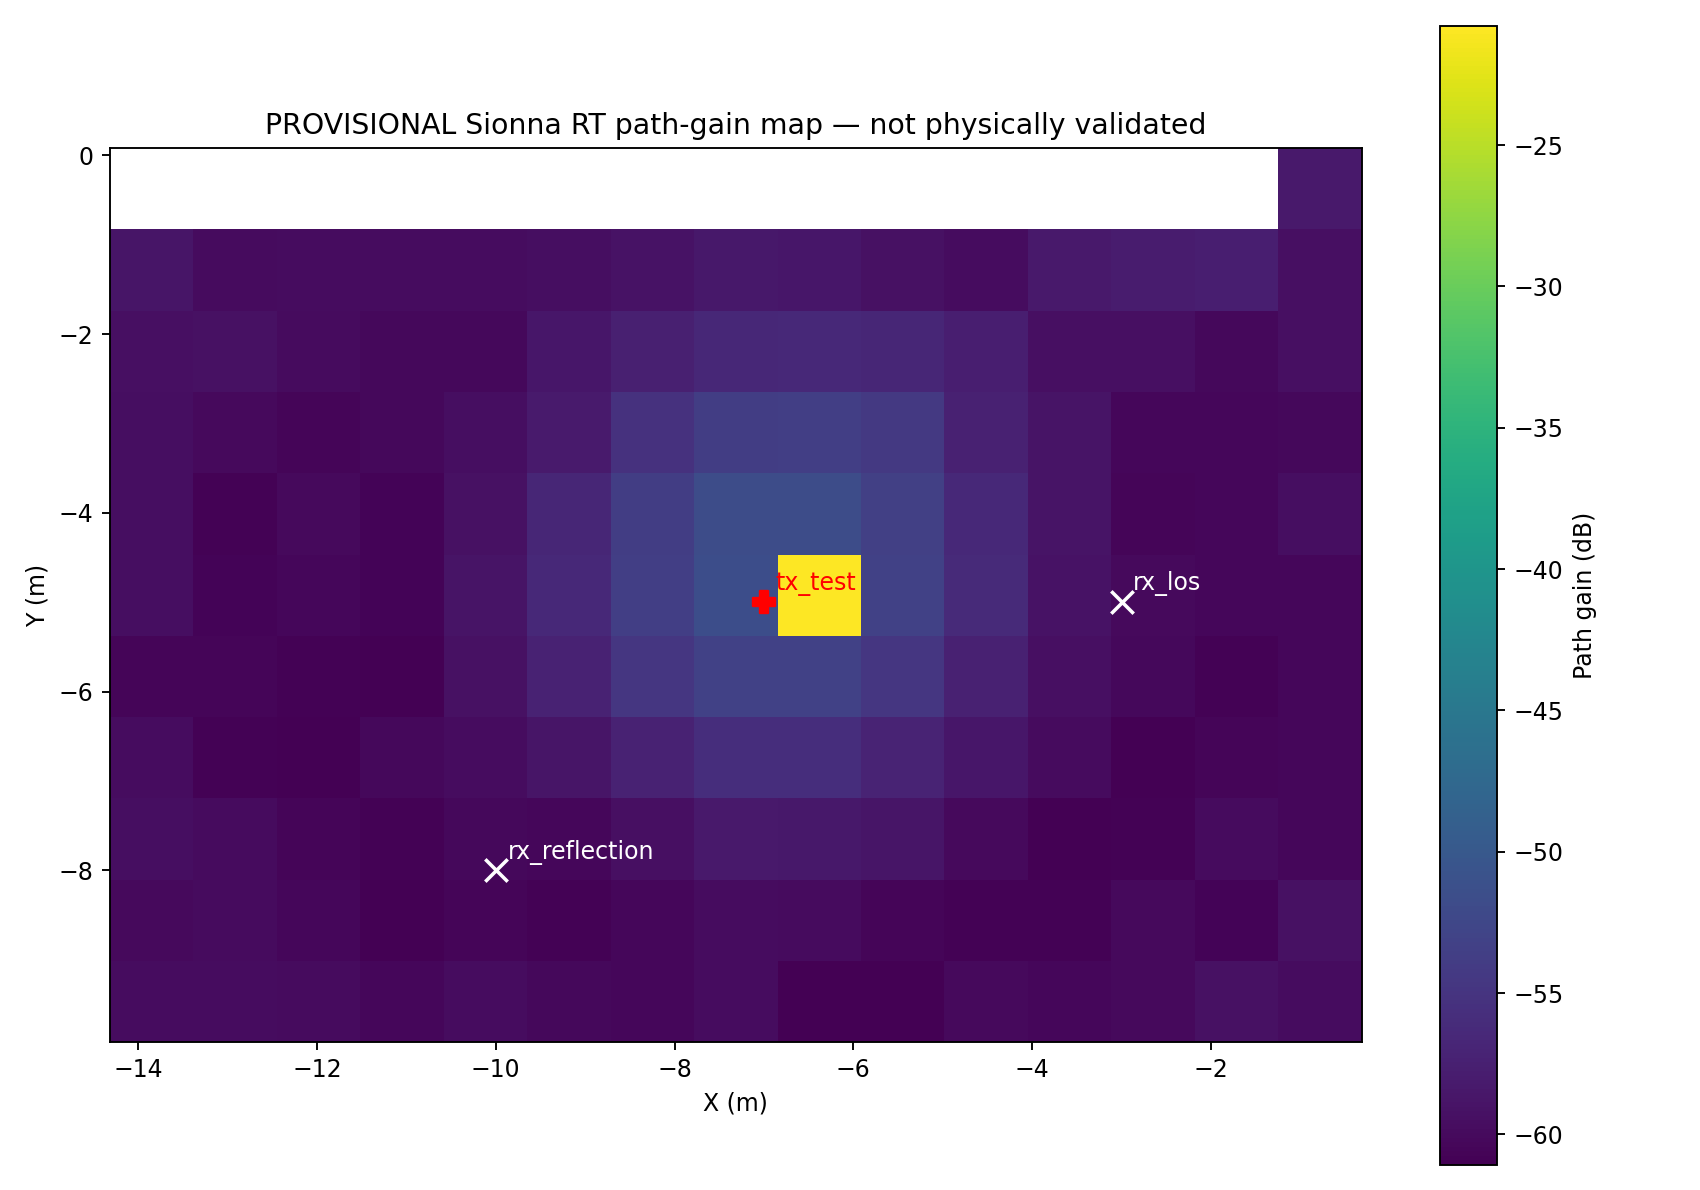
\includegraphics[width=\linewidth]{coverage_baseline.png}
  \caption{가상 벽 없음}
\end{subfigure}\hfill
\begin{subfigure}[b]{0.32\textwidth}
  \centering
  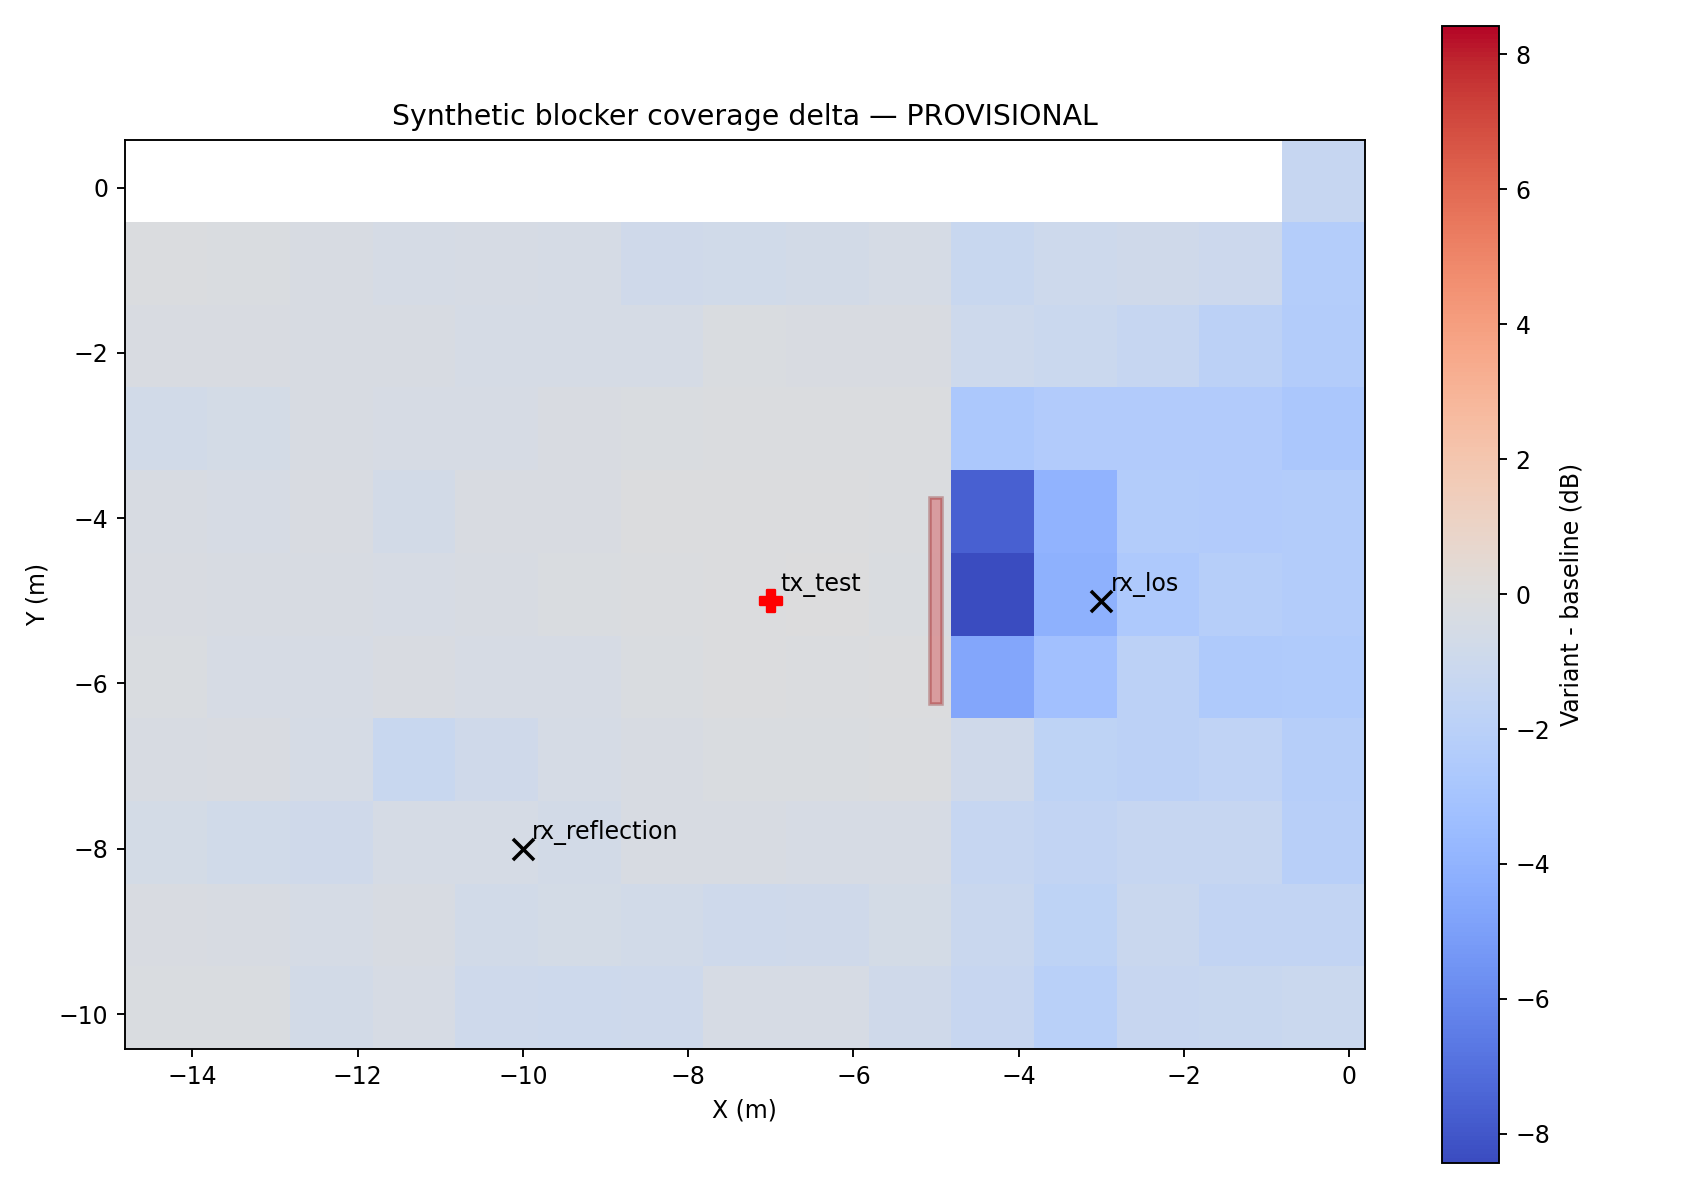
\includegraphics[width=\linewidth]{coverage_delta.png}
  \caption{Variant - Baseline}
\end{subfigure}\hfill
\begin{subfigure}[b]{0.32\textwidth}
  \centering
  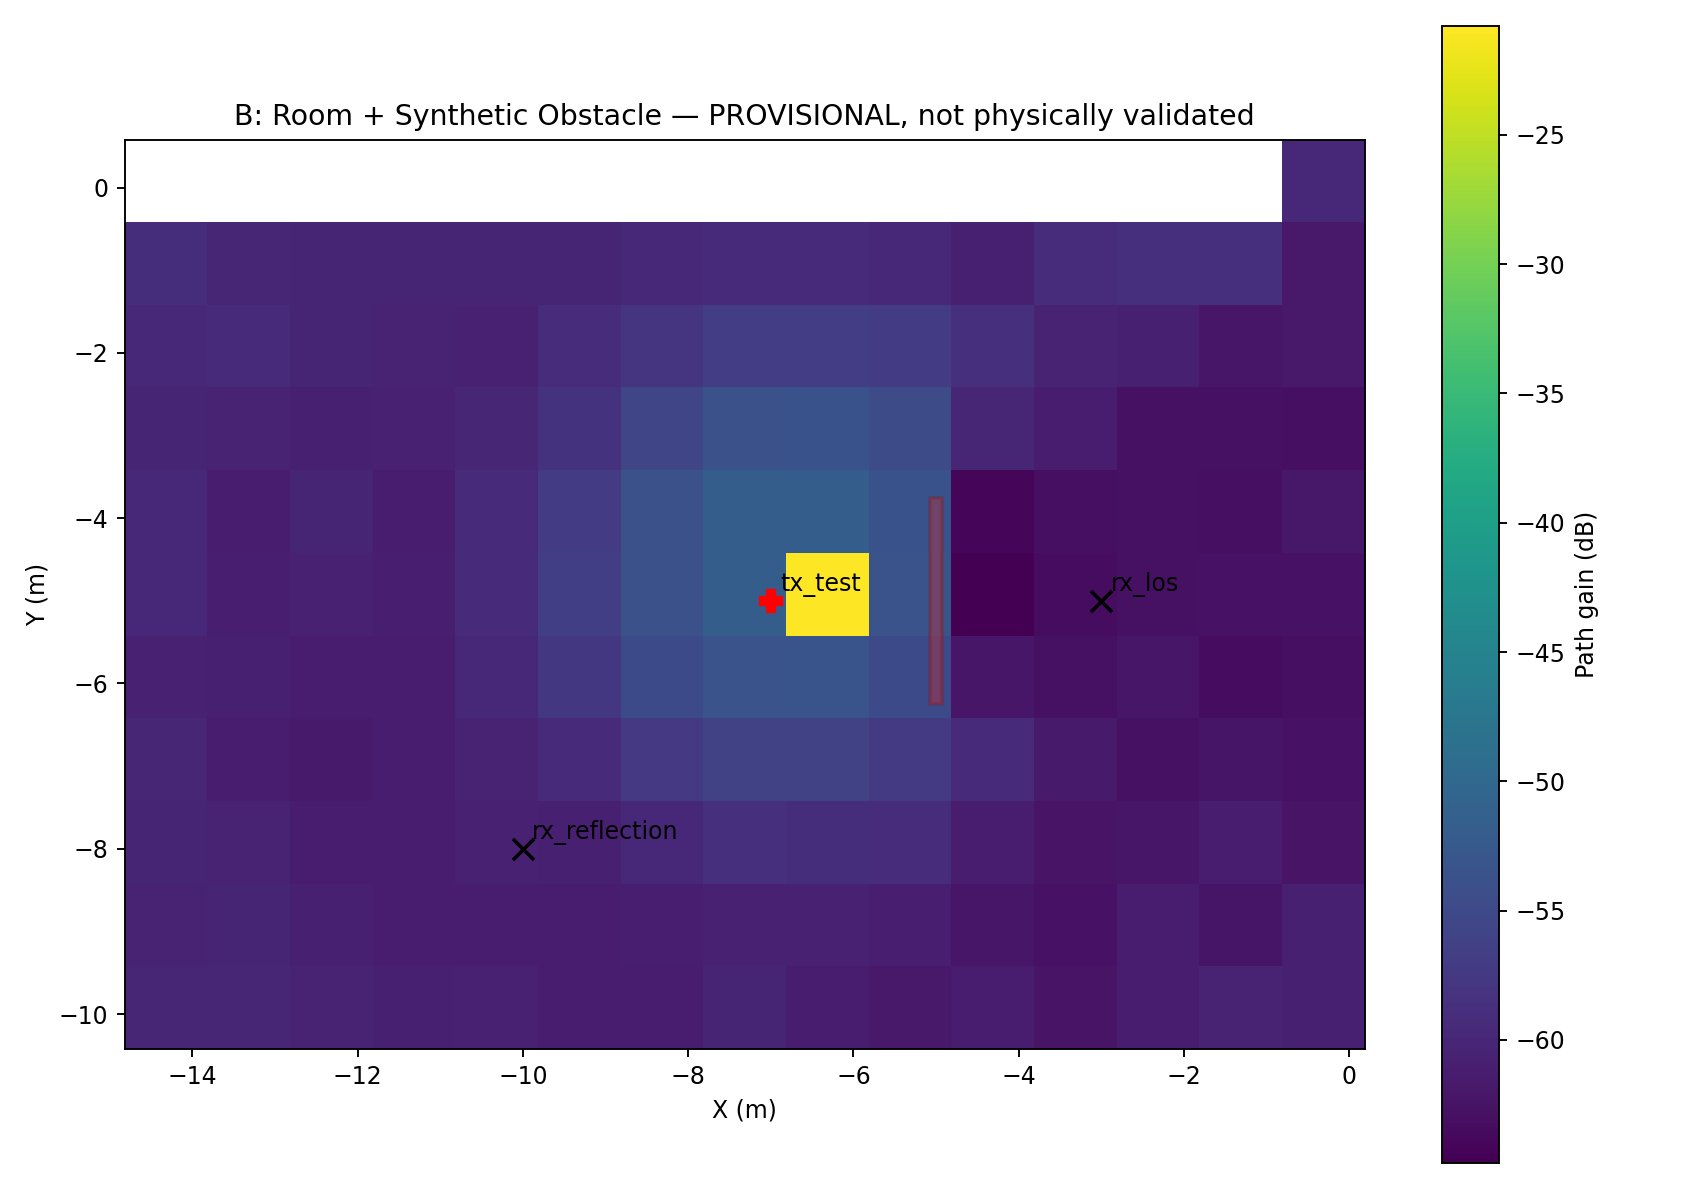
\includegraphics[width=\linewidth]{coverage_variant.png}
  \caption{가상 벽 있음}
\end{subfigure}
\caption{검증용 가상 벽에 따른 전파 지도 A/B 결과. 실제 강의실 구조와 재질을 검증한 수치가 아니라 구조물 반영 경로의 동작 검증이다.}
\label{fig:coverage-ab}
\end{figure}

\begin{figure}[H]
\centering
\begin{subfigure}[b]{0.49\textwidth}
  \centering
  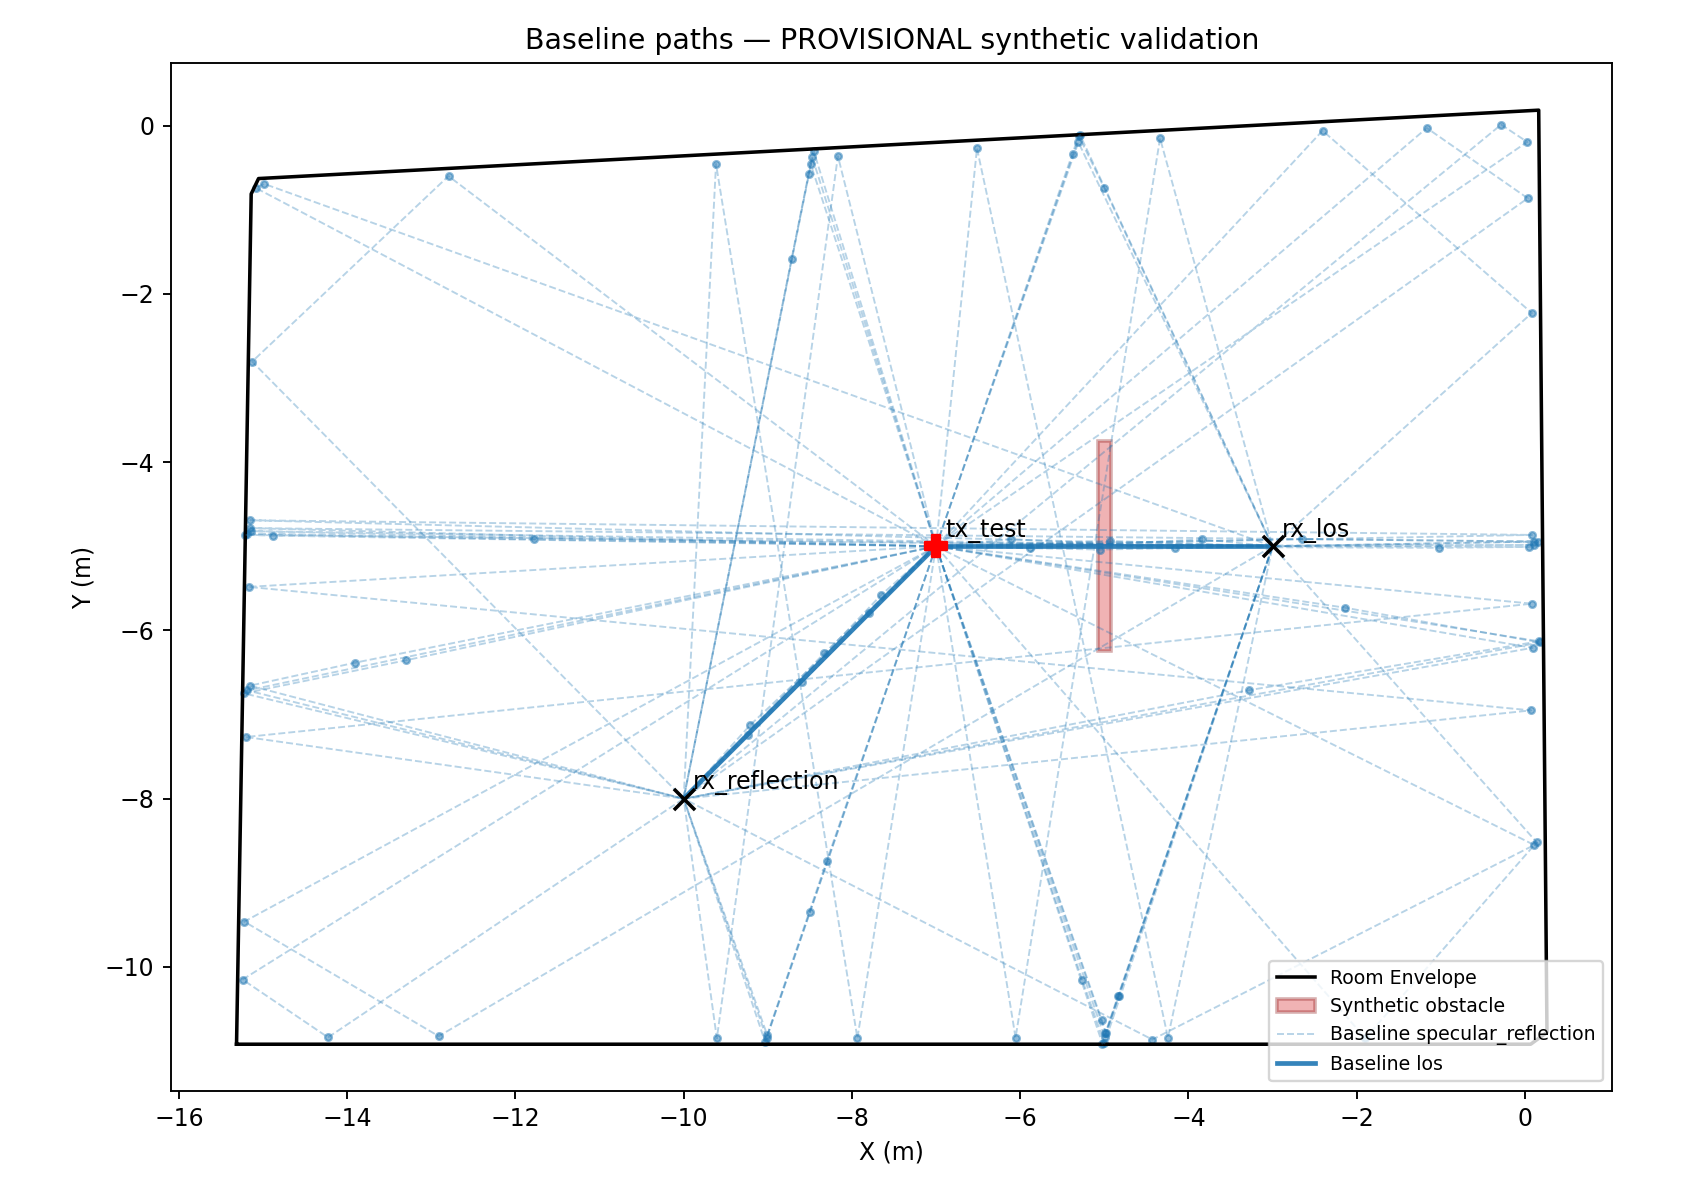
\includegraphics[width=\linewidth]{paths_baseline.png}
  \caption{Baseline 경로}
\end{subfigure}\hfill
\begin{subfigure}[b]{0.49\textwidth}
  \centering
  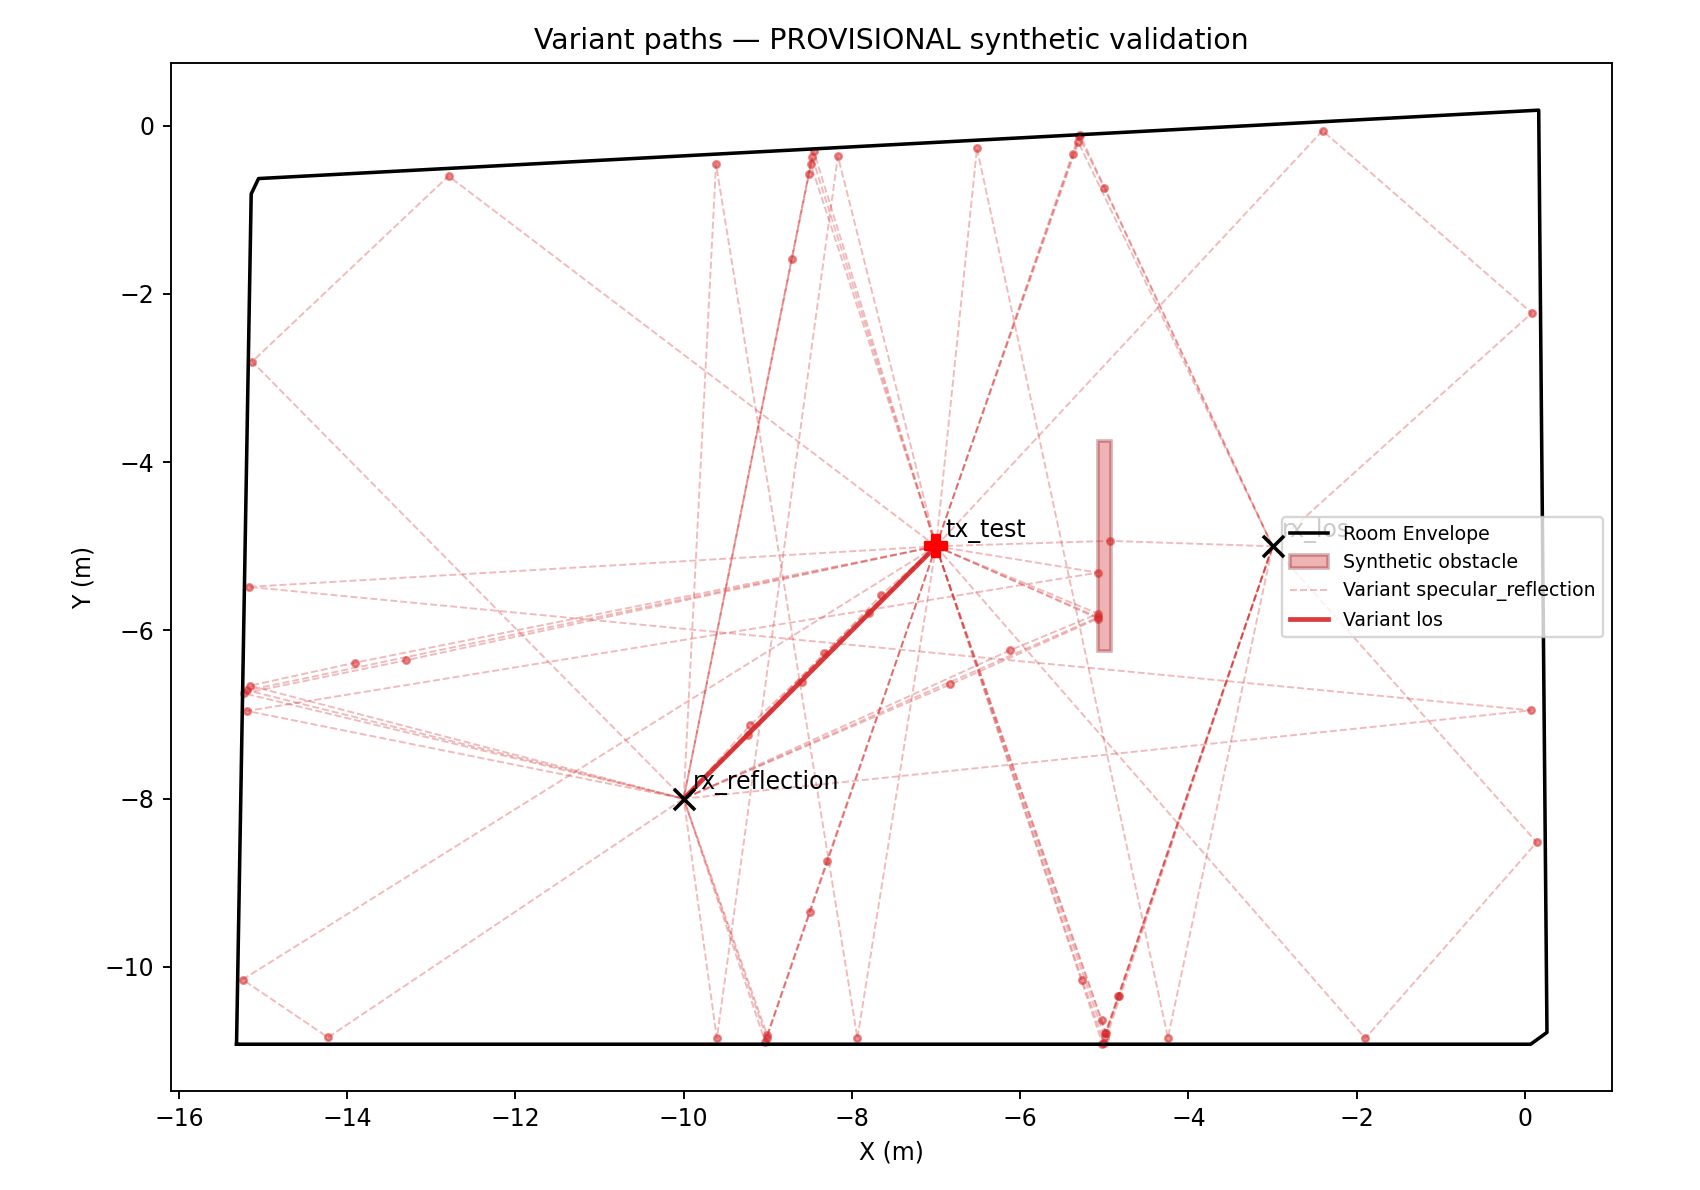
\includegraphics[width=\linewidth]{paths_variant.png}
  \caption{Variant 경로}
\end{subfigure}
\caption{가상 벽 추가 전후의 직접/반사 경로 변화}
\label{fig:path-ab}
\end{figure}

가우시안 자체에서 전파 경로를 계산하는 GaussianRT-RF-NVS는 화면과 전파 계산의 표현을 통합할 수 있는 장기 대안이다\cite{vaara2026gaussianrt}. 그러나 2026년 5월 공개된 초기 연구이고 현재 프로젝트는 이미 PGSR Mesh와 Sionna RT의 연결을 검증했으므로, 중간 단계에서는 현재 경로를 유지하고 비교 연구 대상으로만 둔다.

\section{네트워크 및 백엔드 파트}

\subsection{원격 장치 연결과 데이터 저장}

개발용 브로커에서는 원격 기기의 발행이 백엔드 구독자에게 전달되지 않는 문제가 있었다. 브로커 도청으로 연결과 발행 수신까지는 확인한 뒤 Mosquitto로 교체하였고, 원격 실물 게이트웨이와 로컬 시험 장치의 요청을 동시에 처리하였다. 이후 데이터가 PostgreSQL과 대시보드에 반영되고 WebSocket으로 전달되는 경로를 확인하였다.

\begin{figure}[H]
\centering
\begin{subfigure}[b]{0.49\textwidth}
  \centering
  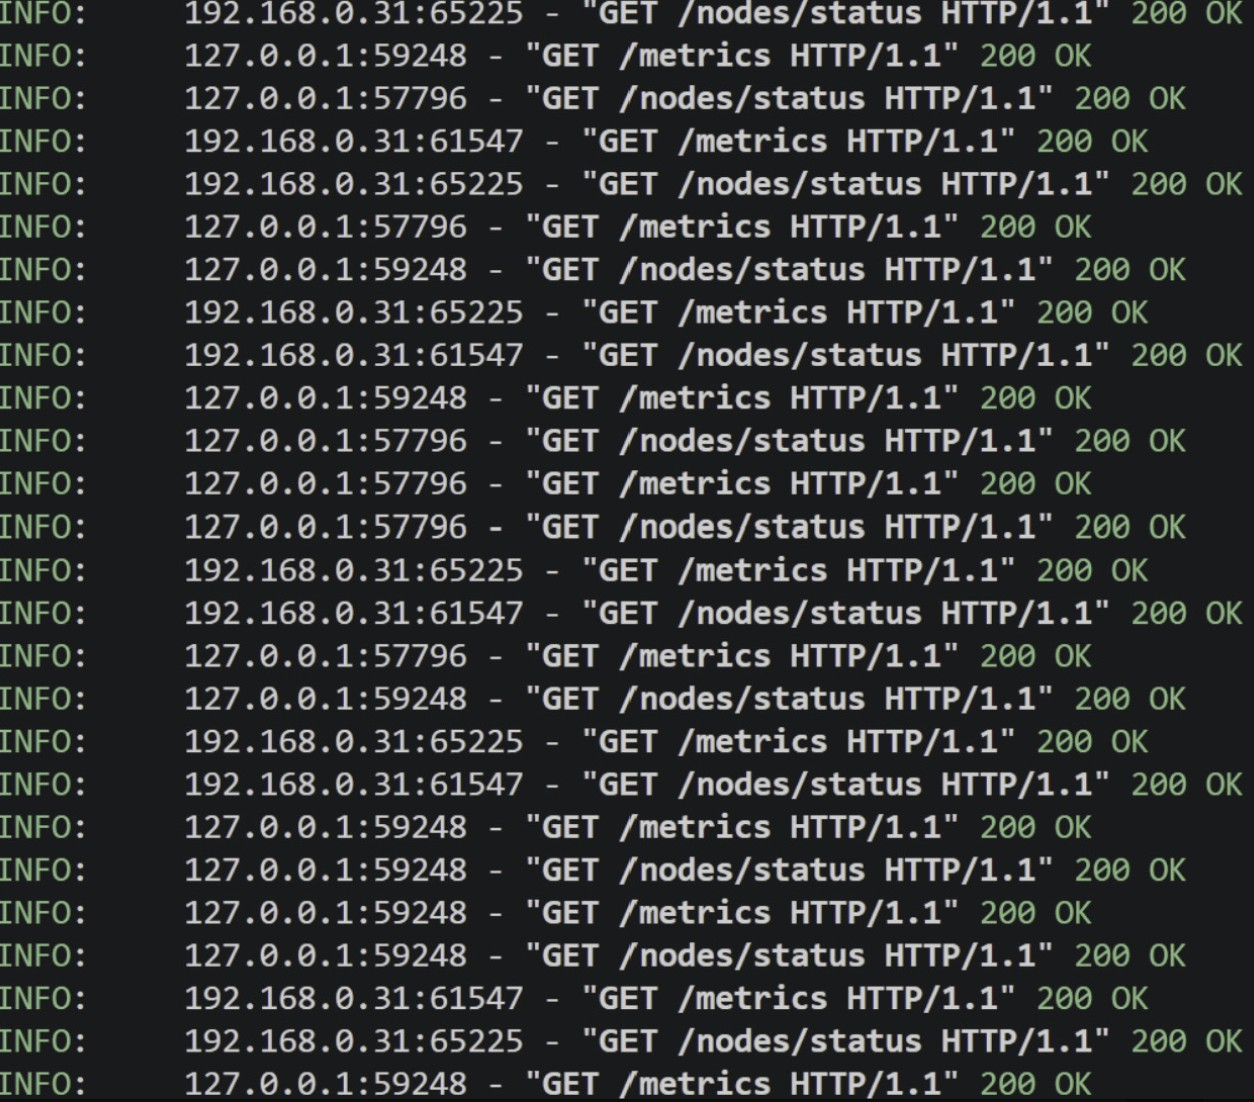
\includegraphics[width=\linewidth]{network_server_log.jpg}
  \caption{원격/로컬 요청 처리 로그}
\end{subfigure}\hfill
\begin{subfigure}[b]{0.49\textwidth}
  \centering
  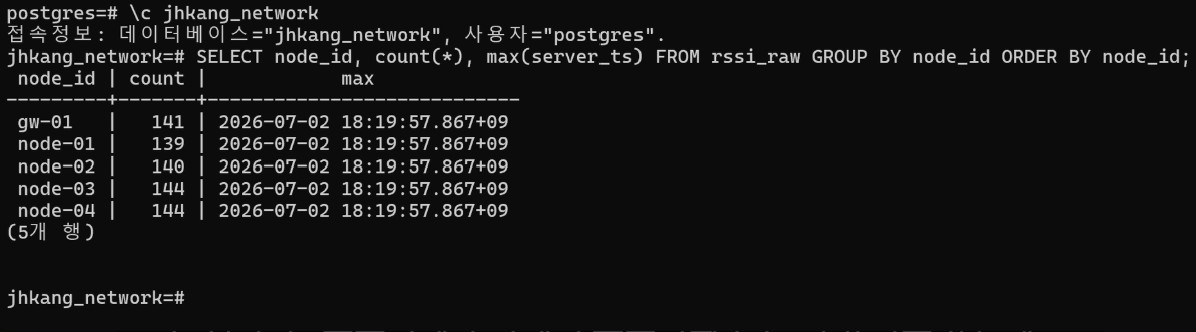
\includegraphics[width=\linewidth]{network_db.jpg}
  \caption{노드별 PostgreSQL 저장 건수}
\end{subfigure}
\caption{실물 임베디드 게이트웨이 연동의 서버 처리와 저장 결과}
\label{fig:network-results}
\end{figure}

노드별 저장 건수는 141, 139, 140, 144, 144건으로 합계 708건이다. 백엔드가 수신한 708건 모두 저장되어 백엔드 내부 드롭률은 0.00\%였고 155개의 동기화 프레임을 생성하였다. 평균 수집 지연은 146.67 ms, p95는 244 ms, 최대는 257 ms였으며 평균 프레임 생성 시간은 5.88 ms였다.

\begin{figure}[H]
\centering
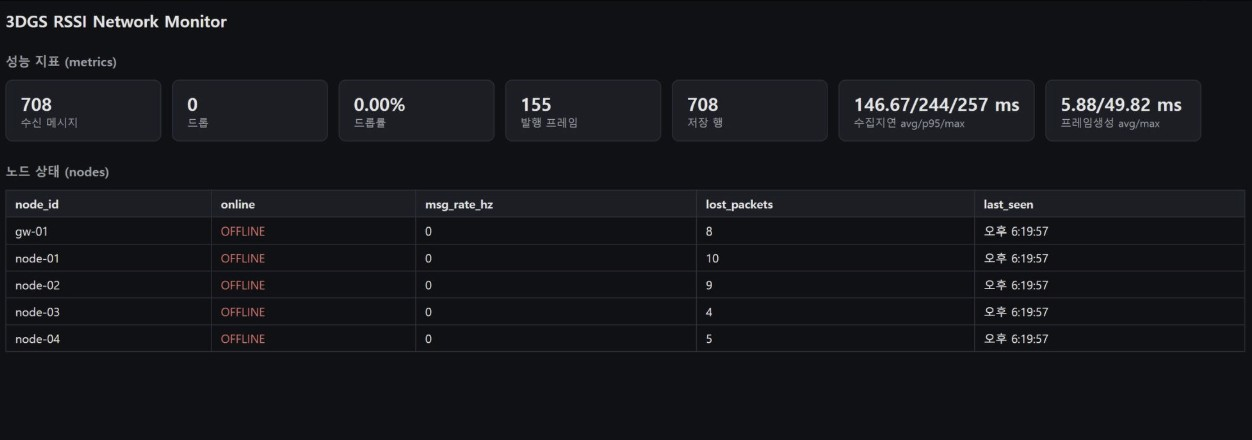
\includegraphics[width=0.96\textwidth]{network_dashboard.jpg}
\caption{실물 데이터 708건 수신 후의 네트워크 모니터링 대시보드}
\label{fig:network-dashboard}
\end{figure}

대시보드의 드롭률 0.00\%는 ``백엔드가 받은 메시지를 처리 중 버리지 않았다''는 뜻이다. 같은 화면의 노드별 \code{lost\_packets}는 송신 측 순번의 증가 기준과 발행 주기로 인해 백엔드 도착 전에 빠진 것으로 추정되는 구간을 뜻한다. 두 지표는 측정 구간과 원인이 다르므로, 현재 결과를 전체 무선 경로의 무손실로 해석하지 않는다.

\subsection{모의 부하 시험}

노드 수를 2개에서 12개까지 늘리고 각 노드가 초당 10회 발행하는 조건으로 백엔드 부하 시험을 수행하였다. 표 \ref{tab:load-test}와 같이 초당 약 120건까지 백엔드 수신 손실은 없었고, 프레임 생성 시간은 평균 약 1.8 ms로 유지되었다.

\begin{table}[H]
\centering
\caption{네트워크/백엔드 모의 부하 시험 결과}
\label{tab:load-test}
\small
\begin{tabular}{rrrrrr}
\toprule
노드 수 & 발행/수신 & 손실률 & 평균 지연 & p95 지연 & 프레임 평균/최대 \\
 & (건) & (\%) & (ms) & (ms) & (ms) \\
\midrule
2  & 398/398     & 0.00 & 68.8 & 125 & 1.7/3.9 \\
4  & 796/796     & 0.00 & 74.0 & 130 & 1.8/3.9 \\
8  & 1,592/1,592 & 0.00 & 81.2 & 128 & 1.8/3.9 \\
12 & 2,388/2,388 & 0.00 & 86.0 & 144 & 1.8/3.9 \\
\bottomrule
\end{tabular}
\end{table}

\section{임베디드 파트}

\subsection{구현 범위}

ESP32 원격 노드는 RSSI 측정, ESP-NOW 송신, 상태 기록을 FreeRTOS Task로 분리하였다. 게이트웨이는 CRC32, 순번 중복/누락, 노드별 최신값을 관리하고 자체 RSSI를 노드 5로 측정한다. STM32는 UART 인터럽트 수신, Line 재동기화, 체크섬/형식 오류 구분, 노드 상태, JSON 생성을 구현하였다. PC 브리지는 과거와 현재 JSON 형식을 모두 처리하고 숫자 노드 ID를 공통 문자열로 바꾸며 설치 좌표를 결합한다.

호스트에서 STM32 파서는 정상 Line, 오류 체크섬 거부, 두 노드 상태 갱신, MQTT-ready JSON 생성을 확인하였다. ESP32 Node binary는 App Partition 약 28\%, Gateway는 약 26\%의 여유를 남기고 빌드되었다. 이 결과는 소프트웨어와 단일 경로의 기본 동작을 입증하지만, 3개 이상 실물 노드의 동시 무선 성능과 장시간 신뢰성을 입증하지는 않는다.

\begin{table}[H]
\centering
\caption{임베디드 모듈별 구현 및 검증 상태}
\label{tab:embedded-status}
\small
\begin{tabularx}{\textwidth}{C{3.0cm}Y C{2.2cm}}
\toprule
모듈 & 보고 시점 결과 & 상태 \\
\midrule
ESP32 RSSI Node & 측정, 5개 이동평균, 1 Hz 패킷, 빌드 성공 & \statuspartial \\
ESP32 Gateway & ESP-NOW 수신, CRC/순번 관리, UART 변환, 빌드 성공 & \statuspartial \\
STM32 Parser & 인터럽트 수신, 체크섬/형식 검사, 호스트 시험 통과 & \done \\
STM32 실물 & J-Link flash 및 실행 성공 이력 & \statuspartial \\
Serial-MQTT Bridge & JSON 정규화, 좌표 결합, MQTT publish 정상 & \done \\
3개 이상 실물 노드 & 보드별 설정과 30분 이상 동시 시험 필요 & \pending \\
장애 대응 & 자동 재연결, Ring Buffer, Watchdog 미구현 & \pending \\
핸드헬드 & IMU, 버튼, UDP pose, LCD/JPEG 미착수 & \pending \\
\bottomrule
\end{tabularx}
\end{table}

\chapter{통합 현황과 중간 평가}

\section{착수 목표 대비 통합 상태}

보고 시점의 가장 중요한 성과는 파트별 코드 존재가 아니라, 실물 임베디드 게이트웨이가 발행한 데이터가 MQTT, 백엔드, PostgreSQL, 대시보드, WebSocket까지 도달하는 경로를 확인했다는 점이다. 그래픽스 파트도 PGSR Mesh에서 Sionna RT Radio Map까지 이어지는 독립 경로를 확인하였다. 그러나 두 경로의 마지막 연결인 ``실측 프레임과 Radio Map을 3DGS Viewer에 합성''하는 기능은 아직 구현되지 않았다.

\begin{table}[H]
\centering
\caption{전체 파이프라인의 중간 통합 상태}
\label{tab:integration-status}
\begin{tabularx}{\textwidth}{C{1.1cm}Y C{2.2cm}Y}
\toprule
단계 & 완료 기준 & 상태 & 현재 근거 또는 남은 검증 \\
\midrule
1 & PGSR 장면과 Mesh 생성 & \done & 사진 205장, 장면/TSDF Mesh 확보 \\
2 & 전파 계산용 닫힌 모델 & \statuspartial & 위상 검증 통과, 실제 배율/재질 미검증 \\
3 & Sionna 경로와 Radio Map & \statuspartial & 직접/반사/가상 벽 A/B 성공, 실제 RSSI 비교 전 \\
4 & 다중 노드 계측 체인 & \statuspartial & 펌웨어/파서/브리지 구현, 3개 이상 장시간 실물 시험 전 \\
5 & 백엔드 저장과 실시간 전달 & \done & 708건 저장, WebSocket/대시보드, 부하 시험 \\
6 & 3DGS와 히트맵 합성 & \pending & SIBR Plane/Depth/합성 구현 필요 \\
7 & IMU 시점과 위치 갱신 & \pending & 센서/알고리즘/인터페이스 시험 필요 \\
8 & JPEG 스트리밍과 LCD & \pending & 인코딩/전송/디코딩/FPS 벤치마크 필요 \\
9 & 전체 시연과 지연 측정 & \pending & 각 계층 통합 후 end-to-end 측정 \\
\bottomrule
\end{tabularx}
\end{table}

\section{검증 결과 요약}

\begin{table}[H]
\centering
\caption{보고 시점의 정량 검증 결과 요약}
\label{tab:quant-summary}
\begin{tabularx}{\textwidth}{C{2.6cm}YY}
\toprule
영역 & 핵심 결과 & 해석 한계 \\
\midrule
그래픽스 기하 & 닫힌 Mesh 8 vertices/12 triangles, 경계/비다양체 0 & 선택 평면과 사진 추정 배율 사용 \\
전파 solver & 내부 151/151셀 유효, 가상 벽 최대 8.426 dB 변화 & synthetic obstacle, 기본 재질, 실측 미비 \\
백엔드 실물 연동 & 708건 수신/저장, 155 frames, 내부 drop 0\% & 송신 구간 seq 누락은 별도 관측 \\
백엔드 부하 & 12 nodes, 약 120 msg/s, 수신 손실 0\% & 모의 발행이며 장기 운전 시험 아님 \\
임베디드 & Node/Gateway build, STM32 host parser 통과, MQTT publish & 다중 실물/장시간/장애 시험 미완료 \\
코드 회귀 시험 & 그래픽스 관련 171 passed, 2 skipped; 네트워크 10 passed & 전용 display/Sionna 시험은 환경 변수와 별도 실행 필요 \\
\bottomrule
\end{tabularx}
\end{table}

\section{현재 위험 요소와 조치 방향}

\begin{enumerate}
  \item \textbf{좌표와 실제 크기 오차}: 현장 치수를 측정해 배율, 축, 원점을 다시 계산하고, 설치 노드 좌표를 동일 기준으로 기록한다.
  \item \textbf{전파 재질과 모델 오차}: concrete/wood 기본값을 확정값으로 사용하지 않고, 실제 RSSI와 시뮬레이션의 위치별 오차를 먼저 비교한다. 필요하면 전역 offset 또는 소수 재질군부터 보정한다.
  \item \textbf{무선/장시간 신뢰성}: BSSID와 채널을 고정하고 3개 이상 노드로 30분, 1시간, 2시간 시험을 수행한다. 재연결 시간, seq 손실, heap, reset reason을 함께 기록한다.
  \item \textbf{Viewer 가림 처리}: 작은 depth bias를 먼저 넣지 않고 카메라 행렬, 좌표계, 실제 크기, Mesh 방향을 검증한다. Mesh depth가 부족할 때만 PGSR unbiased depth를 비교한다.
  \item \textbf{영상 지연 누적}: Render/Encode/Network/Pose Thread를 분리하고, 크기 1--2의 queue에서 오래된 frame을 버린다. 전체 지연뿐 아니라 각 단계 시간을 따로 측정한다.
\end{enumerate}

\chapter{갱신된 추진 계획과 역할 분담}

\section{우선순위 기반 추진 계획}

기존 일정의 병렬 개발 원칙은 유지하되, 최종 통합에 필요한 선행조건을 기준으로 순서를 조정하였다.

\begin{longtable}{C{2.2cm}p{5.5cm}p{4.5cm}}
\caption{보고 이후 갱신된 추진 계획}\label{tab:future-plan}\\
\toprule
기간/우선순위 & 주요 작업 & 완료 판단 기준 \\
\midrule
\endfirsthead
\toprule
기간/우선순위 & 주요 작업 & 완료 판단 기준 \\
\midrule
\endhead
7월 하순 P0 & MQTT topic/payload/QoS 동결, BSSID/게이트웨이 MAC 확정, 3개 이상 노드 실물 동시 시험 & 30분 이상 로그, 노드 ID 유지, 손실/지연 통계, 공통 schema 문서 \\
7월 하순 P0 & 강의실 길이와 주요 물체 실측, 노드 설치 좌표 기록 & 장면-미터 변환 갱신, 좌표 왕복 검증, 설치표 \\
7월 하순 P1 & 재연결, Ring Buffer, Watchdog, 상태 지표 & AP/브로커 중단 후 자동 복구와 1--2시간 연속 시험 \\
8월 초 P0 & SIBR에서 PGSR Gaussian 로드, Heatmap Plane, offscreen final texture & 장면 위 반투명 지도와 좌표 정렬 화면 \\
8월 초 P1 & 실제 RSSI와 Sionna 지도 비교, 단일 보정 기준 검토 & 동일 위치 표본, 오차 표/그림, 과대 해석 없는 결론 \\
8월 중순 P0 & Mesh depth-only pass와 히트맵 가림 처리 & 벽 뒤 히트맵 차폐, 경계 오류 원인 기록 \\
8월 중순 P1 & IMU quaternion 수신, recenter, 버튼식 position update & 방향 반영, 버튼 미입력 시 위치 유지, drift 기록 \\
8월 하순 P1 & JPEG 인코딩, TCP 전송, ESP32-S3 LCD 표시 & 품질별 크기/시간, 5--10 FPS 가능 여부, PSRAM 사용량 \\
9월 P0 & 전체 통합, end-to-end 성능 측정, 시연/문서화 & FPS, 각 단계 지연, 전체 지연, 실패 시 동작과 대안 시연 \\
\bottomrule
\end{longtable}

\section{구성원별 역할과 다음 협업 항목}

\begin{table}[H]
\centering
\caption{구성원별 담당 영역과 후속 작업}
\label{tab:roles}
\begin{tabularx}{\textwidth}{C{2.3cm}C{2.5cm}YY}
\toprule
구성원 & 담당 & 현재 주요 결과 & 다음 협업 항목 \\
\midrule
이승우 & 그래픽스 & PGSR 장면/Mesh, Proxy Mesh, 미터 좌표, Sionna RT A/B & 현장 치수/물체 입력, SIBR 합성, RSSI 비교 \\
강주호 & 네트워크/백엔드 & Mosquitto, 검증/동기화, PostgreSQL, WebSocket, 모니터링 & schema 동결, seq 손실 협의, 인증, 통합 지연 \\
이나영 & 임베디드 & ESP32 Node/Gateway, STM32 파서/JSON, Serial-MQTT Bridge & 실물 다중/장시간 시험, 장애 대응, IMU/LCD \\
공통 & 통합/문서화 & 파트 간 데이터 형식과 1차 실물 연결 & 좌표계 합의, 재현 절차, 성능표, 최종 시연 \\
\bottomrule
\end{tabularx}
\end{table}

\section{미확정 의사결정}

다음 항목은 시험 결과 없이 확정하지 않는다.

\begin{itemize}
  \item 고정 ESP32를 이용한 핸드헬드 위치 추정 방식과 버튼식 Position Snap 알고리즘
  \item 실제 RSSI와 Sionna RT 결과의 결합 또는 보정 방식
  \item IMU yaw drift 보정 방식과 최종 센서 모델
  \item PGSR Mesh depth와 unbiased depth 중 가림 처리 기준
  \item JPEG 품질, 인코더, GPU-CPU 화면 복사, ESP32-S3 buffer 구조
  \item 여러 높이 지도 또는 3차원 volume 표현의 확장 여부
\end{itemize}

\chapter{결론}

본 과제는 착수 단계의 개념 구조를 실제 구현 가능한 두 개의 경로로 구체화하였다. 첫째, 사진 205장으로 만든 PGSR 장면에서 닫힌 전파 계산용 Mesh와 미터 좌표를 만들고 Sionna RT의 경로 및 Radio Map까지 연결하였다. 둘째, ESP32/STM32 계측값이 MQTT, 백엔드, PostgreSQL, WebSocket으로 전달되는 실물 데이터 경로를 구축하였다. 가상 벽 A/B 시험과 네트워크 부하 시험은 각 경로가 구조 변화와 노드 증가에 반응하는지 정량적으로 확인한 중간 성과다.

반면 현재 결과만으로 실제 강의실의 신호 세기를 정확히 예측하거나, 최종 3DGS 화면이 핸드헬드에서 실시간 동작한다고 결론 내릴 수는 없다. 그래픽스의 배율과 재질은 임시값이고, 임베디드는 다중 실물 노드 장시간 시험과 핸드헬드 기능이 남아 있으며, Viewer 합성과 JPEG 스트리밍은 구현 전이다. 따라서 중간 단계의 정직한 결론은 ``핵심 입력과 계산/수집 파이프라인은 확보했으며, 최종 시연을 위한 좌표 보정, Viewer 합성, 장치 안정화가 남았다''는 것이다.

후속 개발에서는 기능 수를 늘리기보다 최종 연결에 필요한 증거를 우선한다. 현장 실측으로 좌표와 물체를 확정하고, 다중 노드의 손실과 재연결을 측정하며, 단일 높이 Radio Map을 SIBR Viewer에 올린 뒤 IMU와 영상 전송을 연결한다. 각 단계는 입력, 출력, 지연, 실패 시 동작을 독립적으로 기록하여 전체 시스템의 병목과 한계를 설명할 수 있는 최종 결과로 발전시킬 예정이다.

\clearpage
\bibliographystyle{plain}
\bibliography{references}

\end{document}
